
\vspace*{-1cm}
\fancyhead[RE, RO]{\fancyplain{}{\small \sl{General startup concepts}}}
\section{General startup concepts}
\label{sec:startup_concepts}
\noindent
\large
As the author already mentioned, the most commonly used software or applications usually do not require any more complex initial setup. However, this may not be the case for GIS software. Therefore, the following subsection introduces and compares several GIS approaches in terms of startup mechanisms. Then we move even beyond GIS and look especially on the way, how software programs chosen according to the first survey enhance the first-time user experience.

\subsection{GIS software}
\label{subsection:GIS software}

The startup mechanisms are analyzed from various perspectives, which are summarized in the final table identifying several questions:
\begin{itemize}
\item Does the GIS software have its own startup screen, and if so, how does it look like? 
\item Does the software have file association of project file?
\item Does the software offer first-time mode to help complete beginners, and if so, in what form?
\item How the software works with data of different coordinate systems? Does it support On the fly transformation? Does it allow the incorrect display of two layers of different coordinate systems on top of each other?
\end{itemize}

\noindent On Figures \ref{fig:hodnoceni_all} and  \ref{fig:hodnoceni_free} we can see graphs of the 10 highest rated GIS software and the 10 highest rated Free GIS software in the world in 2020, as stated in the evaluation taken by online magazine GISGeography. The evaluation of selected software is performed on a point scale from 0 to 10 in four categories - \textit{cartography, analysis, editing and data management} which are subsequently averaged. 

In the first place we can notice two representatives of ESRI - ArcGIS Pro, ArcGIS Desktop. I would also mention the other two interesting commercial software GeoMedia (Hexagon) and MapInfo Professional. If we focus only on Free GIS Software, in the first places in descending order we can find QGIS 3, QGIS 2, gVSIG, GRASS GIS, ILWIS and SAGA GIS. 

\vspace{0.3cm}
\begin{figure}[hbt!] 
\begin{center}
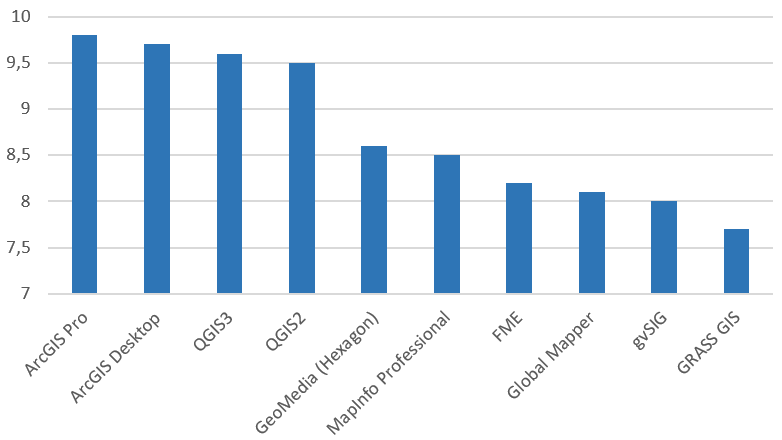
\includegraphics[width=13cm]{../pictures/hodnoceni_all.png} 
\caption[Top 10 GIS Software in 2020 according to GISGeography journal]{Top 10 GIS Software in 2020 according to GISGeography journal}
\label{fig:hodnoceni_all}
\end{center}
\end{figure}

\begin{figure}[hbt!] 
\begin{center}
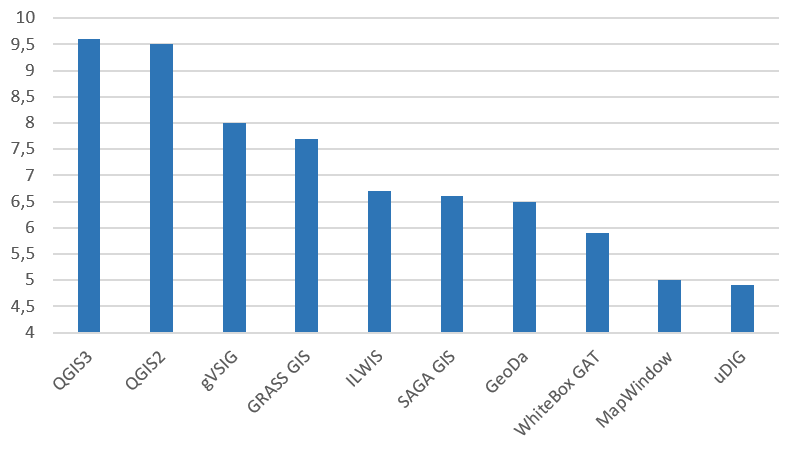
\includegraphics[width=13cm]{../pictures/hodnoceni_free.png} 
\caption[Top 10 Free GIS Software in 2020 according to GISGeography journal]{Top 10 Free GIS Software in 2020 according to GISGeography journal}
\label{fig:hodnoceni_free}
\end{center}
\end{figure}

\newpage
\noindent We must keep in mind that this evaluation is very indicative, as each software has different strengths. For example, on Figure \ref{fig:hodnoceni_analysis} GRASS GIS takes the leading position in then \textit{analysis} category, with a rating of 9.8 out of 10, which is comparable to FME and ArcGIS Pro. Among Free GIS Software GRASS has the highest rating in this aspect. This uniqueness is also mentioned in the pros of the software, which offers more than 350 geoprocessing modules, LiDAR and network analysis, sophisticated tools for satellite imagery, 3D raster rendering and customization and so forth.  The big advantage is that the GRASS GIS function can be leverage through QGIS. 

\newpage
In the disciplines of editing and data management, the balance is somewhat worse 7.4 and 7.5 out of 10 points. The biggest drop to 6.1 is in the \textit{cartography} category. At this point, however, it must be highlighted that the ambition of GRASS GIS is definitely not to create high-quality modern maps, but to offer the software for very numerically complex geographical analyzes. What is mentioned as other disadvantages is clunky and dated user interface, defining projects on start-up, steep learning curve to get started and command line window running in background. We can notice that these shortcomings are largely related to the current unfortunate startup mechanism.

\begin{figure}[hbt!] 
\begin{center}
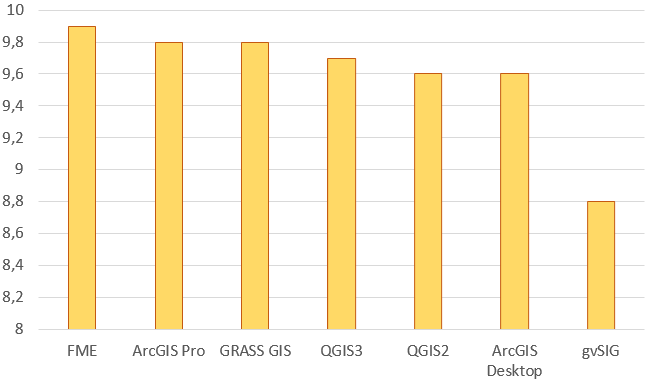
\includegraphics[width=11cm]{../pictures/hodnoceni_analysis.png} 
\caption[Top 7 GIS Software in 2020 in \textit{analysis} category according to GISGeography journal]{Top 7 GIS Software in 2020 in \textit{analysis} category according to GISGeography journal}
\label{fig:hodnoceni_analysis}
\end{center}
\end{figure}

\noindent At this point, it is important to emphasize that in this work we do not focus at all on the functionality of the software as such. As you could read in the previous lines, in this aspect the software is really very different. Therefore, even though the software may not be very user-friendly, a user will have no choice and reach for it. In this work, software is tested and analyzed in detail from the point of view of the startup mechanism and data organization with an emphasis on finding out what elements they use directly in the software to improve the first-time user experience.

The software is tested using two shapefiles of different coordinate system - districts in the Czech Republic in the S-JTSK Krovak East North system (EPSG: 5514) and US tracts in the USA Contiguous Albers Equal Area Conic system (ESRI: 102003). These systems are not selected by chance. They are defined entirely differently, however, in terms of coordinate digits they are very similar.

The author has extensive experience with ArcMap and QGIS, with other software she had the honor of working for the first time. However, for the purposes of this work, this fact is a plus, as the evaluation of software is not distorted by any previous experience.

\newpage
\vspace*{-1cm}
\subsubsection{Analysis of selected commercial software}

\noindent On further rows three commercial representatives (ArcGIS Pro, MapInfo Professional and GeoMedia Advantage) are described in terms of startup mechanisms, new user friendliness and data organization. Data import is also tested for each software. 

\bigskip

\noindent \textbf {ArcGIS Pro 2.4}

\noindent This software is currently the lead representative of ESRI's desktop GIS. It is an extension and connection of ArcMap, ArcScene and ArcGlobe applications. It is therefore possible to display and analyze 3D data in it. After logging in, the startup screen is displayed (see Figure \ref{fig:arcgis_startup_screen}). Here we can open recently saved projects or select from pre-prepared templates, of which we have several to choose from - Map (standard), Catalog, Global scene and Local scene. Another option is to select an empty sheet.

\vspace{0.3cm}
\begin{figure}[hbt!] 
\begin{center}
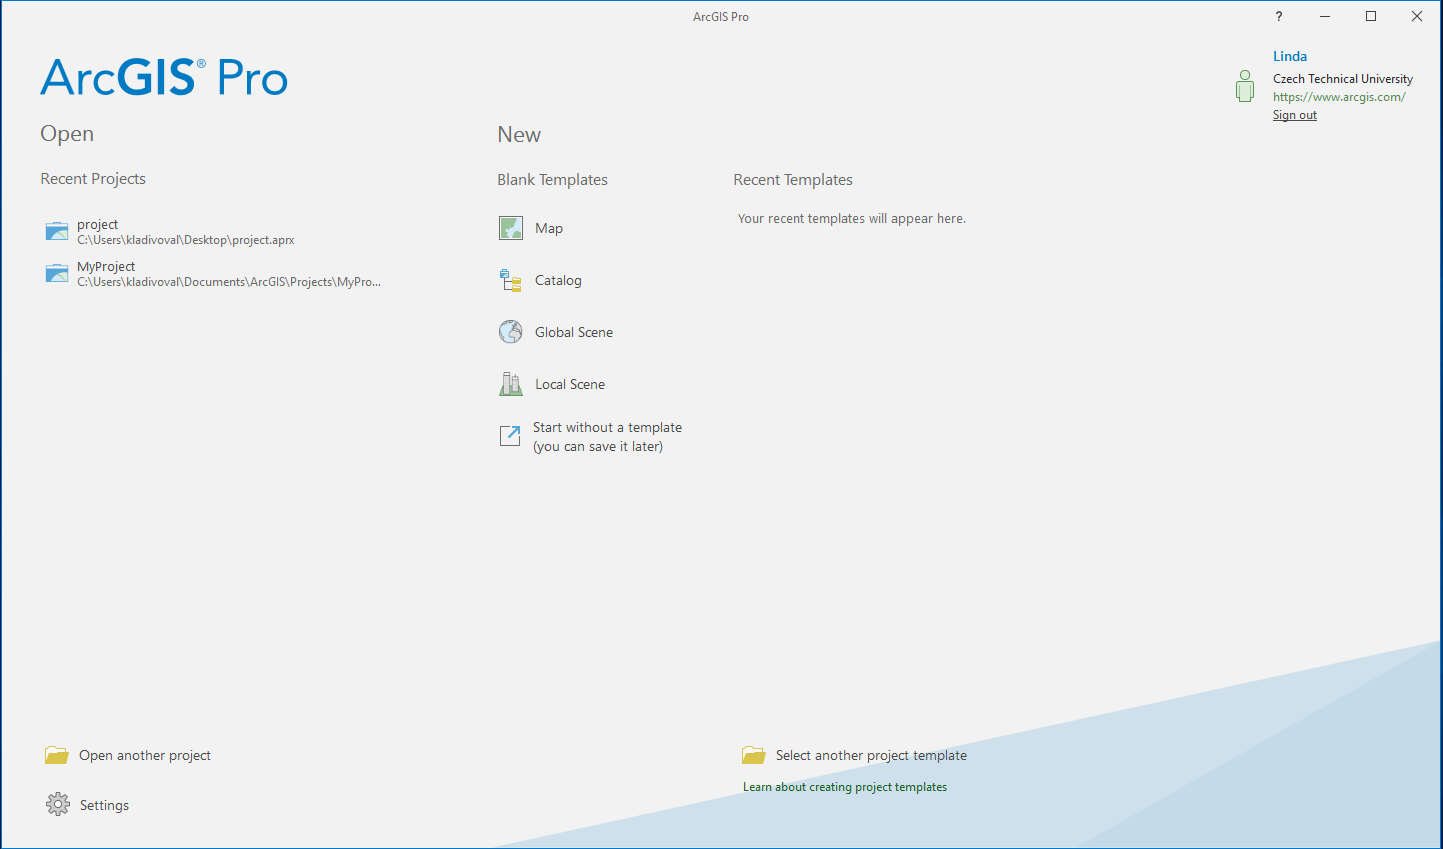
\includegraphics[width=16cm]{../pictures/arcgis_startup_screen.png} 
\caption[ArcGIS Pro 2.4 startup dialog]{ArcGIS Pro 2.4 startup dialog (Source: Personal collection)}
\label{fig:arcgis_startup_screen}
\end{center}
\end{figure}

\noindent The imported GIS layers are located in the Map component which is associated with Map window. In the following example on Figure \ref{fig:arcgis_pro_onthefly2}, the map window system is WGS 1984 Web Mercator Auxiliary Sphere (according to the first added layer), but the later layers added are in other coordinate systems. In spite of having different coordinate systems, the layers are displayed correctly in the map window due to On the fly transformation.

\newpage
\begin{figure}[hbt!] 
\begin{center}
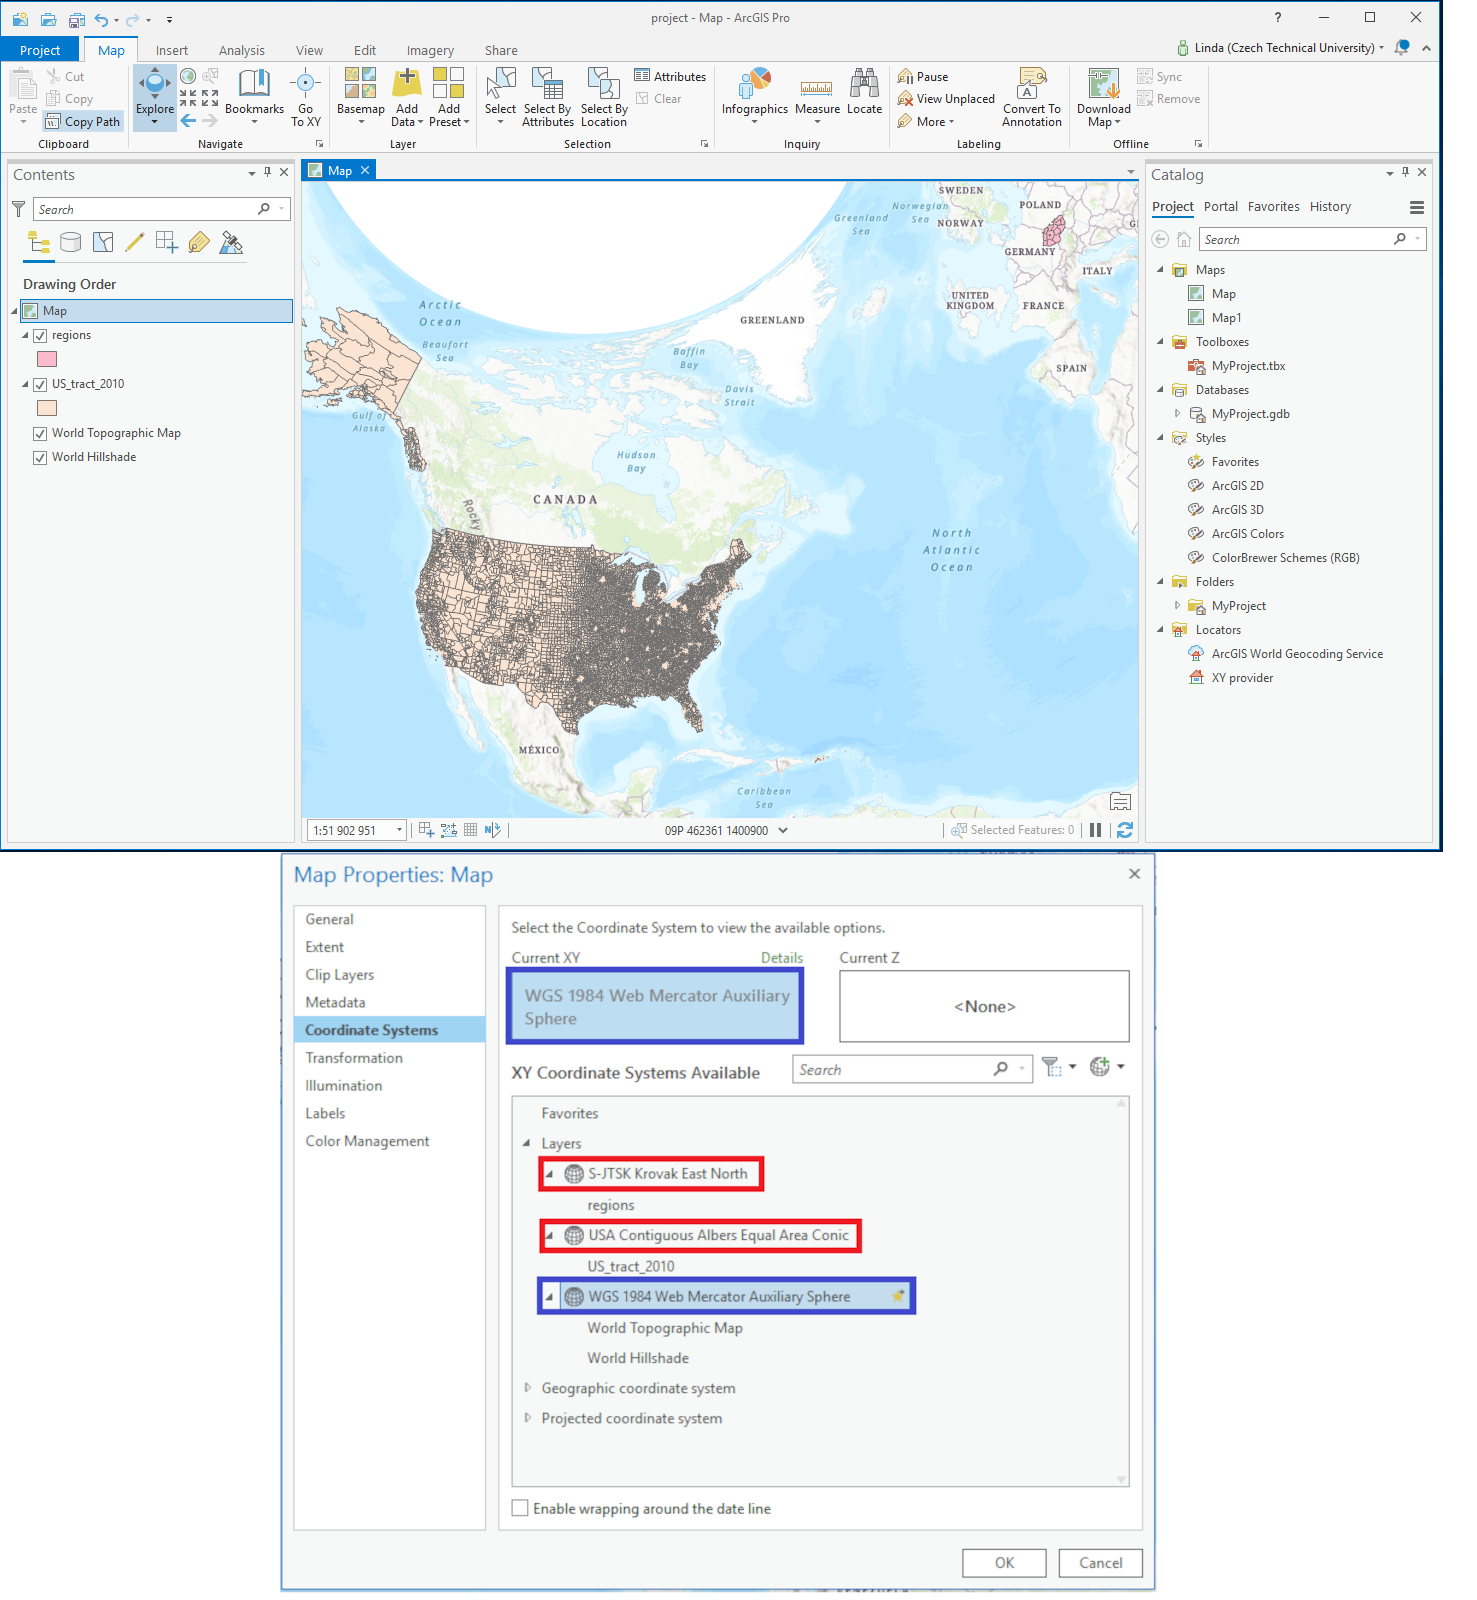
\includegraphics[width=16cm]{../pictures/arcgis_pro_onthefly2.png} 
\caption[Display of layers with different coordinate system in ArcGIS Pro 2.4]{Display of layers with different coordinate system in ArcGIS Pro 2.4 (Source: Personal collection)}
\label{fig:arcgis_pro_onthefly2}
\end{center}
\end{figure}

\noindent ArcGIS Pro works with projects as key elements of data organization. Each project contains a folder that contains the data we want to work with. So there is pressure to make data clear and not scattered all over the disk. We can say that ESRI is moving in a similar direction to GRASS GIS in this aspect. In the case of this software, it is not a disadvantage that it does not offer any special elements or explanations that could help newcomers. The startup screen and the software as such are at first glance clear and user friendly.

\newpage
\vspace*{-1cm}
\bigskip
\noindent \textbf {GeoMedia Advantage 2020}

\noindent This commercial GIS software developed by Intergraph (now Hexagon Geospatial) has a rich 40-year history. It is especially strong at cartography and raster analysis.  It also offers a unique 3D experience for viewing and analyzing data.

After complicated license setup (it is not possible to simply try the trial version, it is necessary to apply for a time-limited license key), we are greeted by a small start dialog captured in Figure \ref{fig:geomedia_startup}, where we can create our own GeoWorkspace file or open an existing one.

\vspace{0.3cm}
\begin{figure}[hbt!] 
\begin{center}
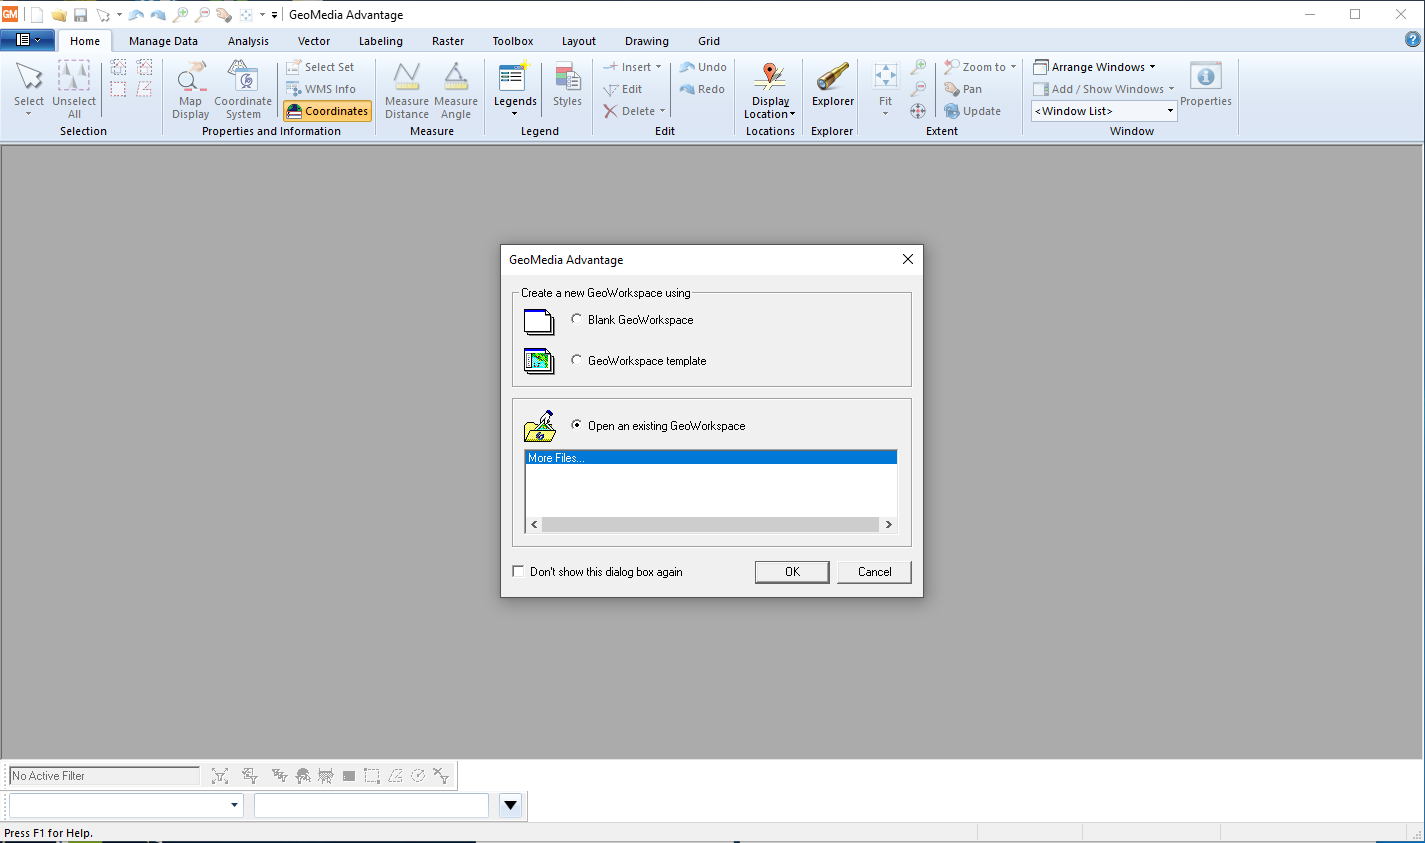
\includegraphics[width=17cm]{../pictures/geomedia_startup.png} 
\caption[GeoMedia Advantage 2020: startup dialog]{GeoMedia Advantage 2020: startup dialog (Source: Personal collection)}
\label{fig:geomedia_startup}
\end{center}
\end{figure}

\noindent Fortunately, the software provides two examples of GeoWorkspaces which give a user at least a little idea of how it all works. However, if we want to add our own data, it is very user-unfriendly and the author managed to do it after half an hour of intensive efforts.

Any external data we want to add to the software has a character of Warehouses. For example, to be able to display shapefiles (but also other formats), a user has to first define a Warehouse Configuration File. It consists of a data server definition (in the case of ArcView shapefile), a working folder with data and a coordinate system definition, see Figure \ref{fig:define_config_geomedia}. GeoMedia, like GRASS, also requires the definition of CRS right at the beginning and provides detailed settings for this purpose.

\vspace{0.3cm}
\begin{figure}[hbt!] 
\begin{center}
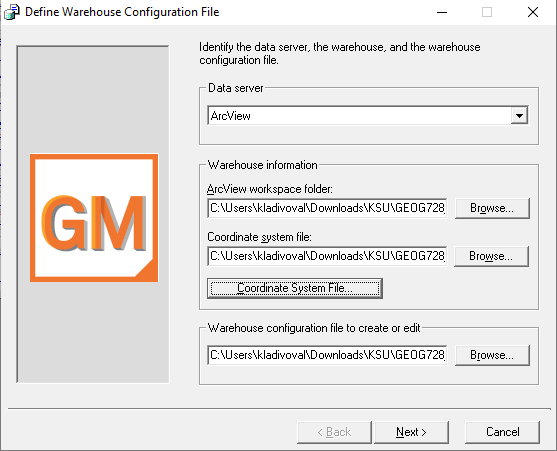
\includegraphics[width=13cm]{../pictures/define_config_geomedia.png} 
\caption[GeoMedia Advantage 2020: Define Warehouse Configuration File dialog]{GeoMedia Advantage 2020: Define Warehouse Configuration File dialog (Source: Personal collection)}
\label{fig:define_config_geomedia}
\end{center}
\end{figure}

\noindent In the next step it is needful to connect this configuration file. Once it is connected we can manipulate with data in a map window as with legend entries. Each GeoWorkspace file can have multiple Warehouses with different coordinate systems attached. In the map window, an On the fly transformation takes place according to the coordinate system of the map window, which is set under the term Location.

The software does not provide any help, so the user is completely clueless and forced to search the Internet. From a learning point of view, this software is definitely the most difficult to understand from the three selected commercial software. However, we can perceive a certain similarity with GRASS, especially in the setting of the coordinate system, which is also very important from the point of view of GeoMedia software. However, the map window supports the On the fly transformation, which is a significant difference from GRASS GIS.

\newpage
\vspace*{-1cm}
\bigskip

\noindent \textbf {MapInfo Professional 2019}

\noindent This commercial GIS software is developed by the American company Pitney Bowes, in the Czech Republic the exclusive provider is CS Map. As the name suggests, MapInfo is very strong in geodata visualization. it offers functionalities for doing modern cartography - several prepared map layouts, advanced labelling, accessing symbology etc. However, some analytical functions e. g. focused on LiDAR and remote sensing are missing.

When we run the software, we are redirected to the startup screen, which atypically occupies the size of the entire computer screen. The startup provides links to new version news or links to videos on YouTube that can help first-time users. In the upper right part of the startup screen it is possible to run help, which has the character of a separate desktop application. In the left part there is a simple bar allowing to choose a workspace we want to work in. We can open an empty workspace, sample workspace with a map of Washington DC or choose another previously saved workspace in the directory path. If we run the software again, the Open Last Saved Session option will be added to the startup screen.

\vspace{0.3cm}
\begin{figure}[hbt!] 
\begin{center}
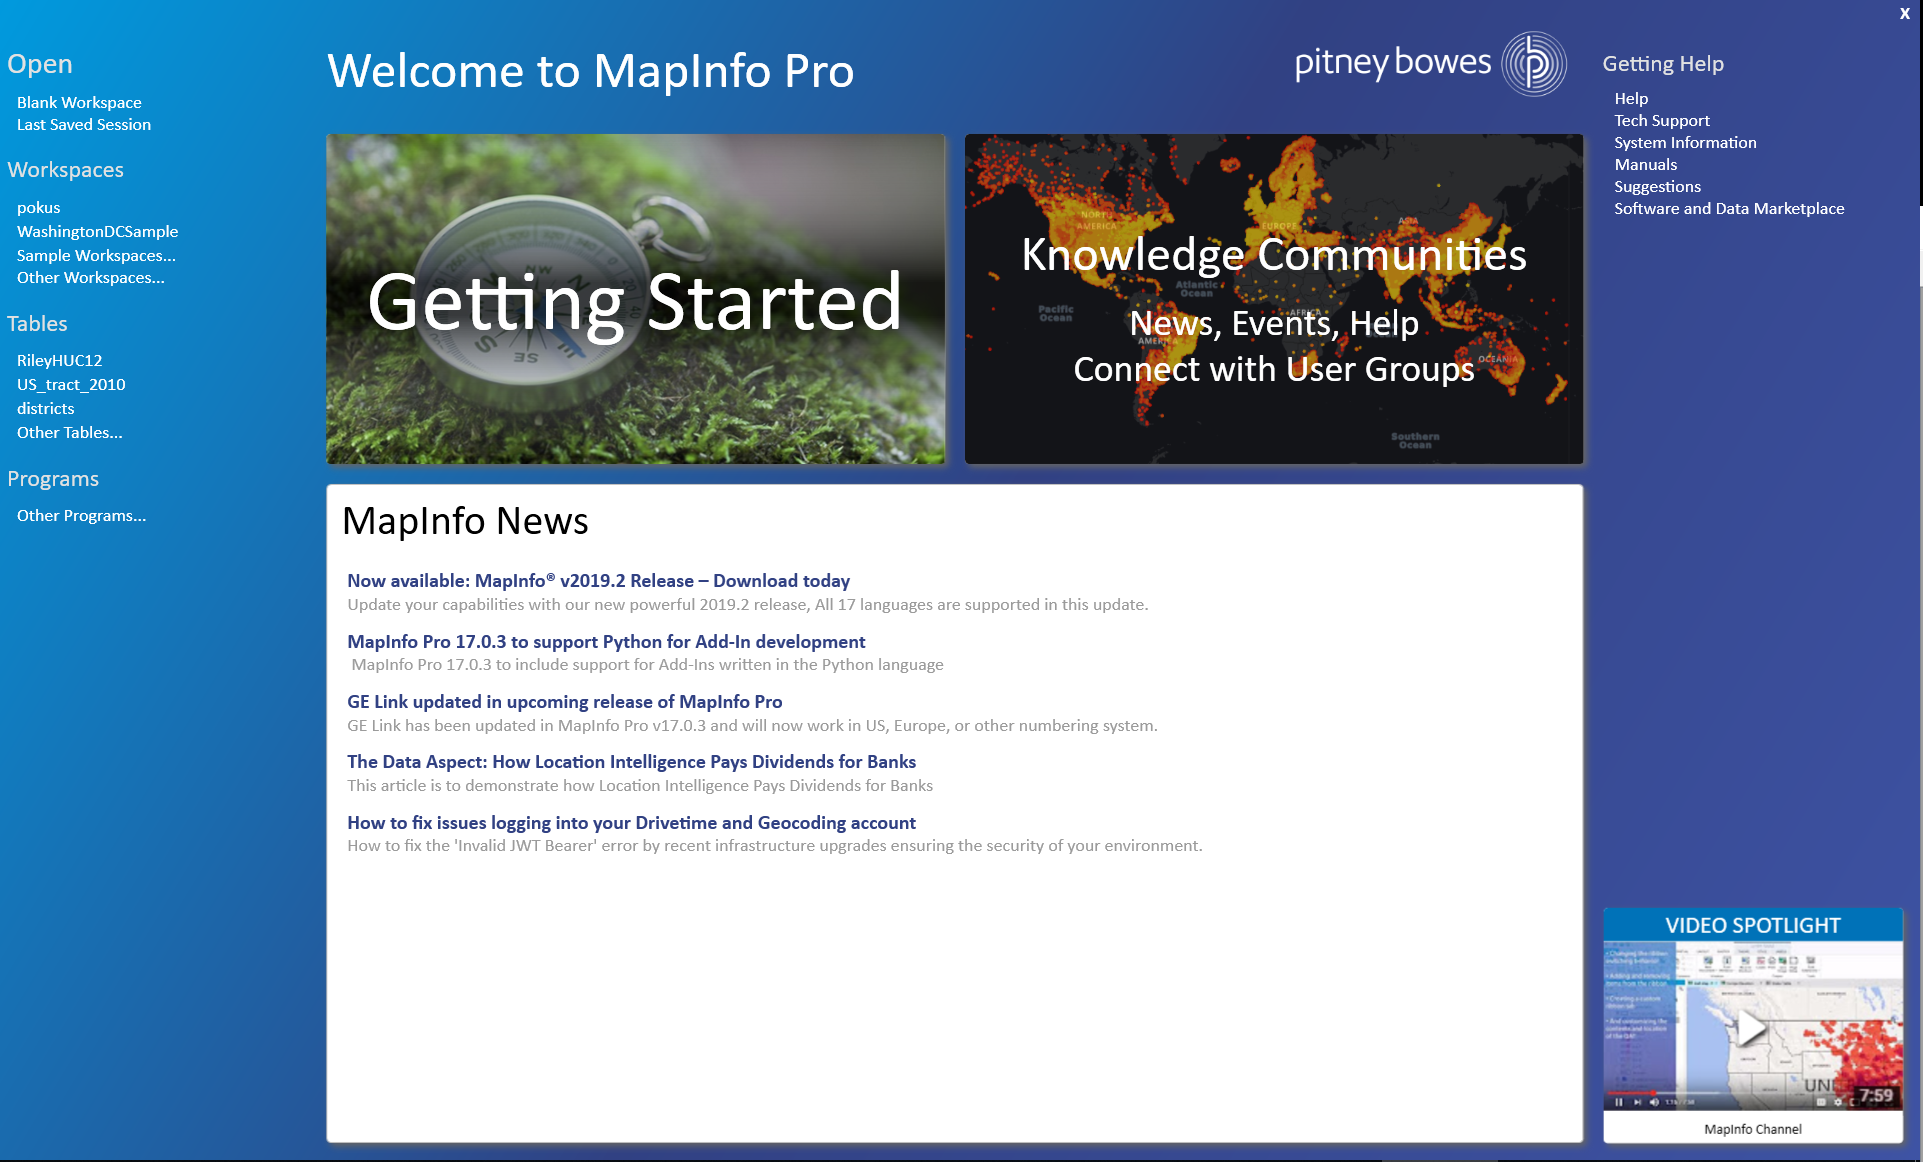
\includegraphics[width=16cm]{../pictures/map_info_startup_screen.PNG} 
\caption[MapInfo Professional 2019 startup dialog]{MapInfo Professional 2019 startup dialog (Source: Personal collection)}
\label{fig:map_info_startup_screen}
\end{center}
\end{figure}

\noindent As in ArcGIS Pro, the main component is the Map, which has one coordinate system defined. Data import is somewhat non-intuitive and must be demonstrated through the Open Table icon. When importing, a new file of company's own geodata format * .tab is created. We can define new projection or keep the original one. Coordinate system of the Map can be changed through Map Options as shown on Figure \ref{fig:map_info_startup_projection}. 

\vspace{0.3cm}
\begin{figure}[hbt!] 
\begin{center}
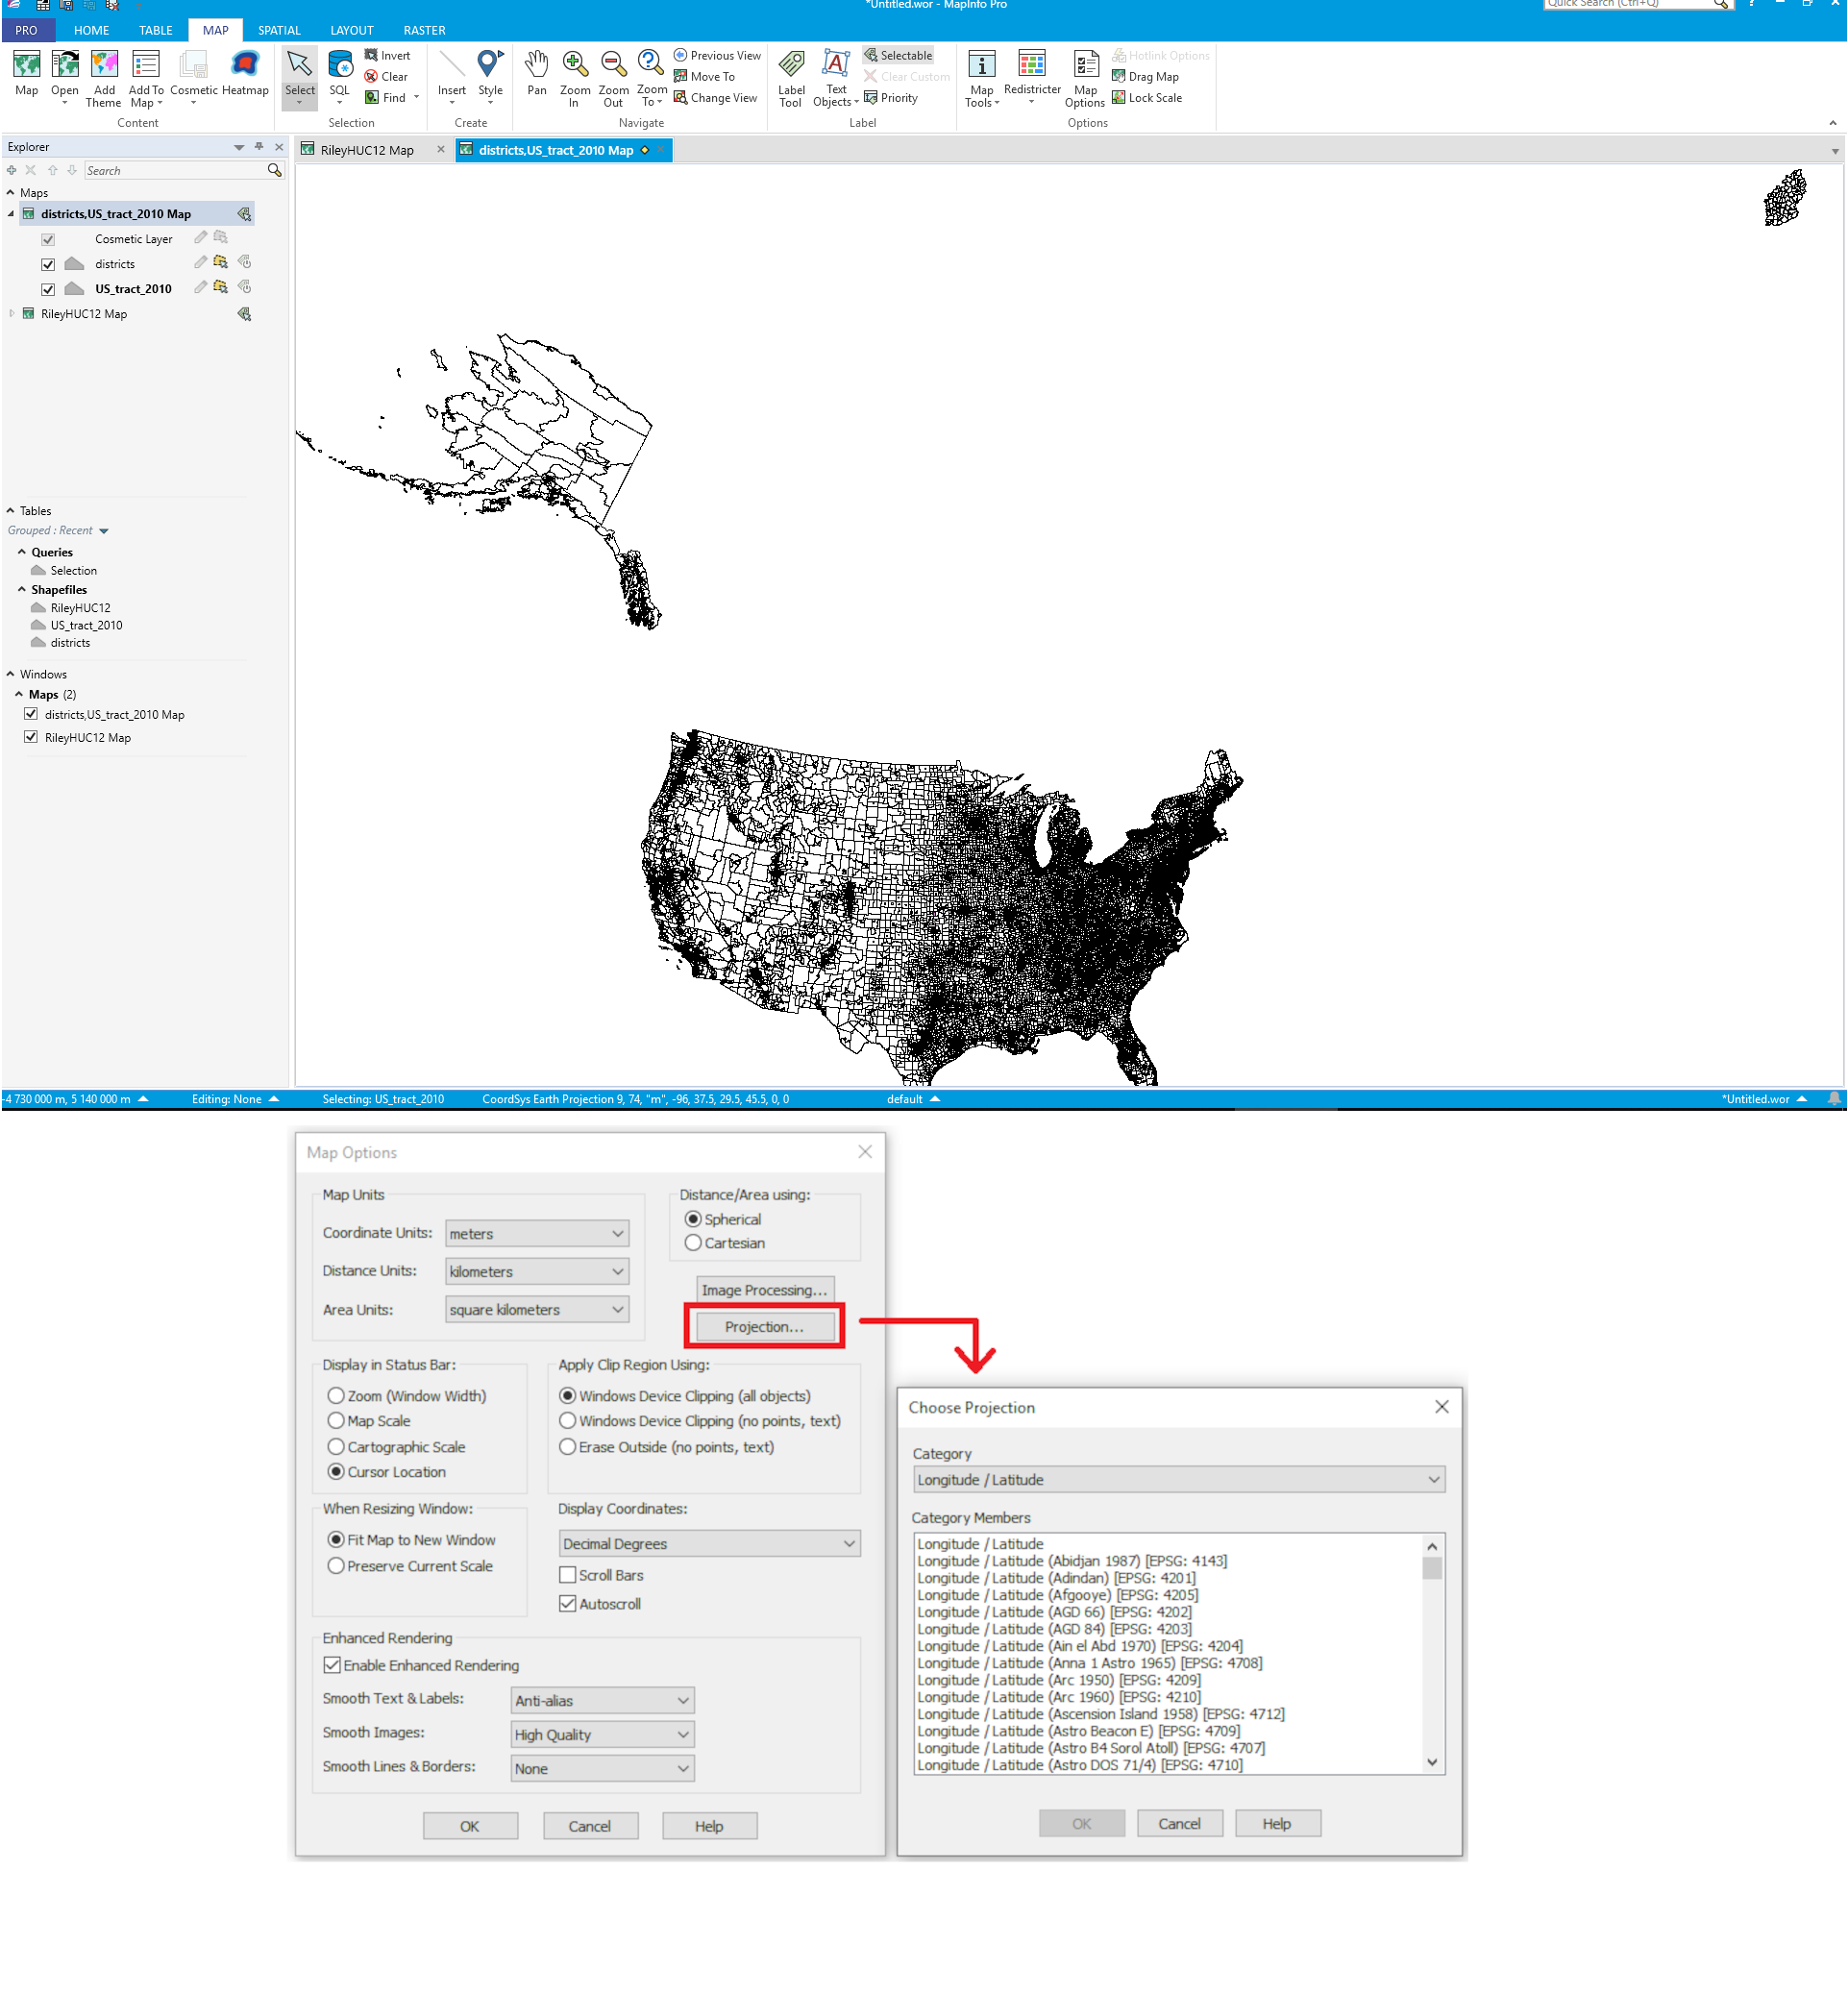
\includegraphics[width=16cm]{../pictures/map_info.PNG} 
\caption[Map-level coordinate system settings in MapInfo Professional 2019]{Map-level coordinate system settings in MapInfo Professional 2019 (Source: Personal collection)}
\label{fig:map_info_startup_projection}
\end{center}
\end{figure}

\noindent However, at first glance it is not clear in which coordinate system the layers are, more precisely whether we made On the fly transformation or data transformation. After a longer examination, it is clear that we transformed MapInfo *.tab file. The coordinate system is set to the map level (not layer level) and takes over the system of the first map layer added. 

\newpage
\vspace*{-1cm}
\subsubsection{Analysis of selected open-source software}

\noindent On further rows four open-source software (QGIS 3, gvSIG, ILWIS, SAGA GIS) are tested and analyzed in detail from the point of view of the startup mechanism with an emphasis on finding out what elements they use directly in the software to improve the first-time user experience. In the next chapter, the results of these analyzes are summarized in tables.

\bigskip

\noindent \textbf {QGIS 3.14}

\noindent This software is created similarly to GRASS GIS under the auspices of OSGeo. The big change from QGIS 2 is that it includes native support for 3D visualizations. The advantage is also the possibility of using and creating tailor-made plugins. QGIS also allows the use of analytical functions from GRASS, SAGA GIS software and the GDAL library. 

At the first start, Welcome to QGIS window appears, in which we can link to the QGIS website and check the news in the given version. The window runs in the default language of the operating system.

\vspace{0.3cm}
\begin{figure}[hbt!] 
\begin{center}
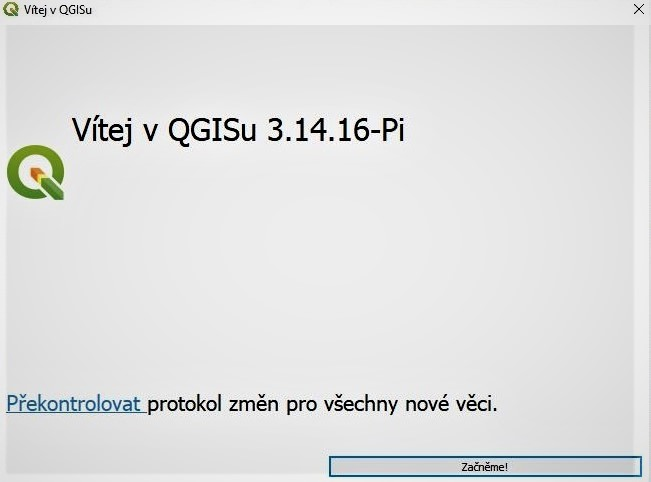
\includegraphics[width=8cm]{../pictures/qgis_startup_window.JPG} 
\caption[Welcome to QGIS 3.14 window]{Welcome to QGIS 3.14 window (Source: Personal collection)}
\label{fig:qgis_startup_window}
\end{center}
\end{figure}

\noindent After this introduction, we are redirected to the main software window (Fig. \ref{fig:qgis_first_window})  informing about community events and significant improvements that have taken place. Here we can choose an empty project template or we may open sample datasets (North Carolina, South Dakota, Alaska) provided along with instalation.

In QGIS 3, we distinguish between the layer's and project's CRS. It is worth mentioning that QGIS supports about 2700 known coordinate systems, whose definitions are stored in the SQLite database installed together with QGIS. The empty project has always global default projection EPSG: 4326 - WGS 84.

\vspace{0.3cm}
\begin{figure}[hbt!] 
\begin{center}
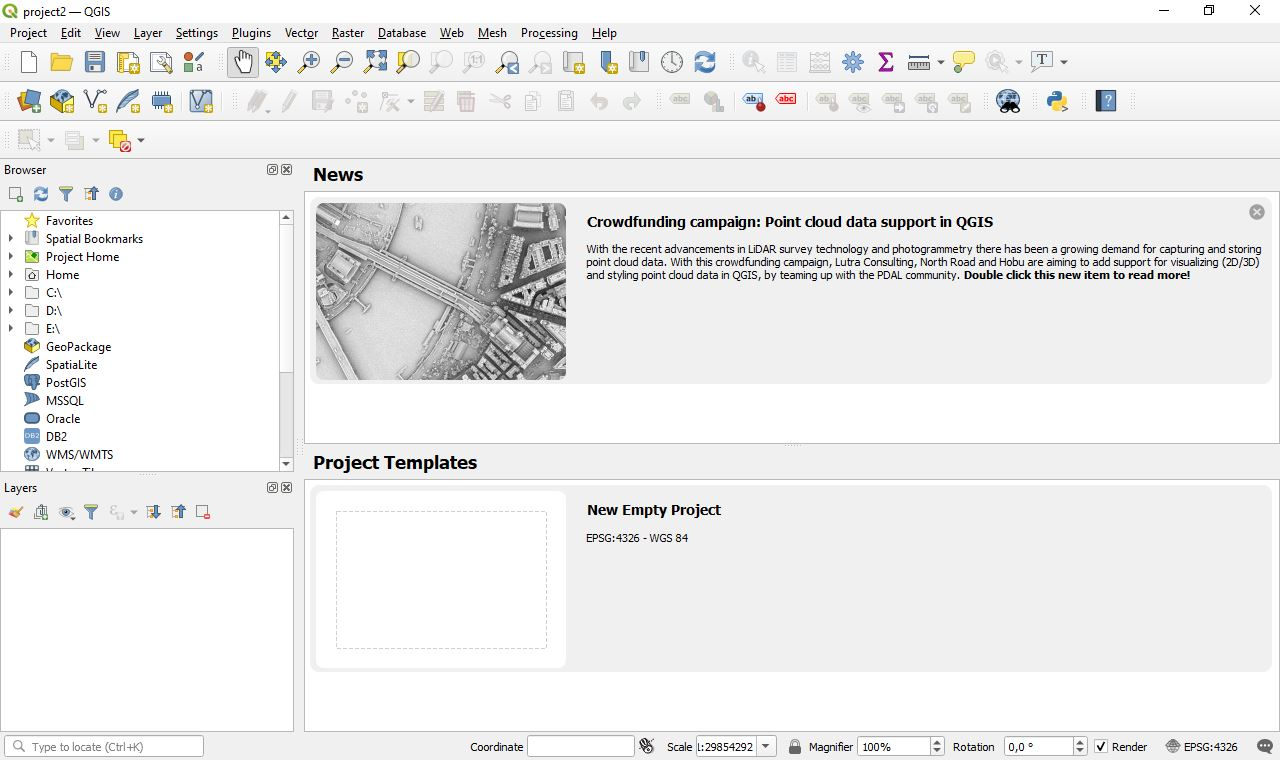
\includegraphics[width=17cm]{../pictures/qgis_first_window.JPG} 
\caption[The main software window after first opening QGIS 3.14]{The main software window after first opening QGIS 3.14 (Source: Personal collection)}
\label{fig:qgis_first_window}
\end{center}
\end{figure}

\noindent In QGIS, On-the-fly transformation is enabled by default, meaning that whenever you use layers with different coordinate systems QGIS transparently reprojects them to the project CRS. When importing the first layer (in this case US tracts in ESRI: 102003 system), the dialog box shown in Fig. \ref{fig:qgis_transformation} specifies what type of transformation to perform when changing the project CRS. These Datum transformations are then listed in Project Properties - CRS settings (Fig. \ref{fig:qgis_trans}). It is important to note that the first layer added defines the coordinate system of the project. In our case, it was changed to the US Contiguous Albers Equal Area Conic system. In the dialog \ref{fig:qgis_trans} we can set the Predefined coordinate system, which is related to the project, not to the layer.

Whenever a more accurate transformation is available, but is not currently usable, QGIS 3 shows an informative warning message (see Fig. \ref{fig:qgis_warning_window}) advising to use more accurate transformation. Those messages appear quite often in a variety of situations, which can definitely help new as well as experienced QGIS users.

\begin{figure}[hbt!] 
\begin{center}

\includegraphics[width=17cm]{../pictures/qgis_warning_window.JPG} 
\caption[Informative warning message  in QGIS 3.14]{Informative warning message  in QGIS 3.14 (Source: Personal collection)}
\label{fig:qgis_warning_window}
\end{center}
\end{figure}

\begin{figure}[hbt!] 
\begin{center}
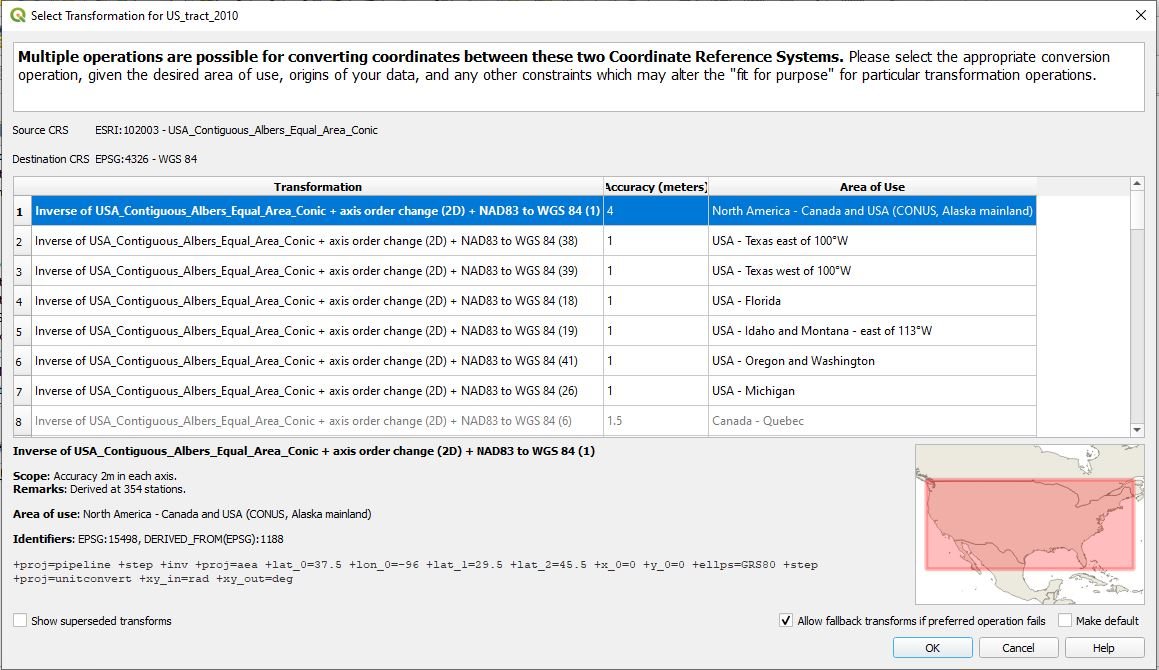
\includegraphics[width=14cm]{../pictures/qgis_transformation.JPG} 
\caption[Select the type of transformation in QGIS 3.14]{Select the type of transformation in QGIS 3.14 (Source: Personal collection)}
\label{fig:qgis_transformation}
\end{center}
\end{figure}

\begin{figure}[hbt!] 
\begin{center}
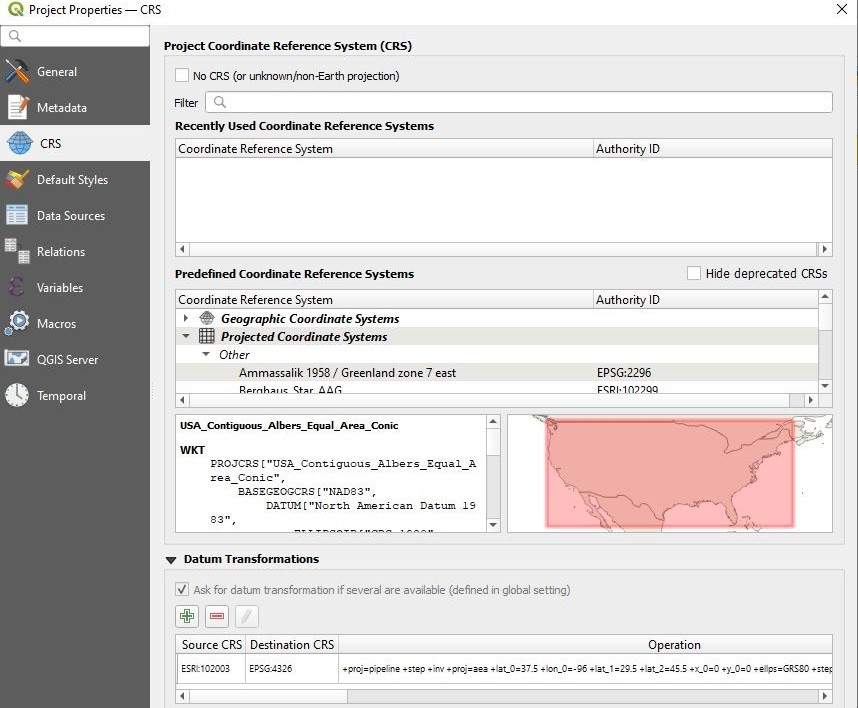
\includegraphics[width=14cm]{../pictures/qgis_trans.JPG} 
\caption[Predefined CRS and Datum Transformations in QGIS 3.14]{Predefined CRS and Datum Transformations in QGIS 3.14 (Source: Personal collection)}
\label{fig:qgis_trans}
\end{center}
\end{figure}


\newpage
\vspace*{-1cm} 
\bigskip

\noindent \textbf {gvSIG 2.5.0}

\noindent Here we will describe the startup mechanism of another open-source software created under the OSGeo organization. gvSIG can work with common vector and raster data, integrates files and databases as well as remote data through OGC standards. It is developed in Java and, like QGIS, includes a plugin system which allows to easily extend the software capabilities and develop tailor-made solutions.

Software is designed very simply. It does not have a startup window, nor does it support any first-time mode. When started, an empty map window will open. The work is saved in a project with the extension * .qvsproj, which can then be started through the associated icon. If we do not start the software using the project's association icon, it is reopened by default with a blank map. Adding layers is also intuitive. It is possible to add multiple layers in different coordinate systems, the software recognizes the EPSG codes. The data still retains its original coordinate system, however, map layers are rendered in the WGS 84 (EPSG:4326) using On the fly transformation, see Fig. \ref{fig:gvSIG_coords}.

\vspace{0.3cm}
\begin{figure}[hbt!] 
\begin{center}
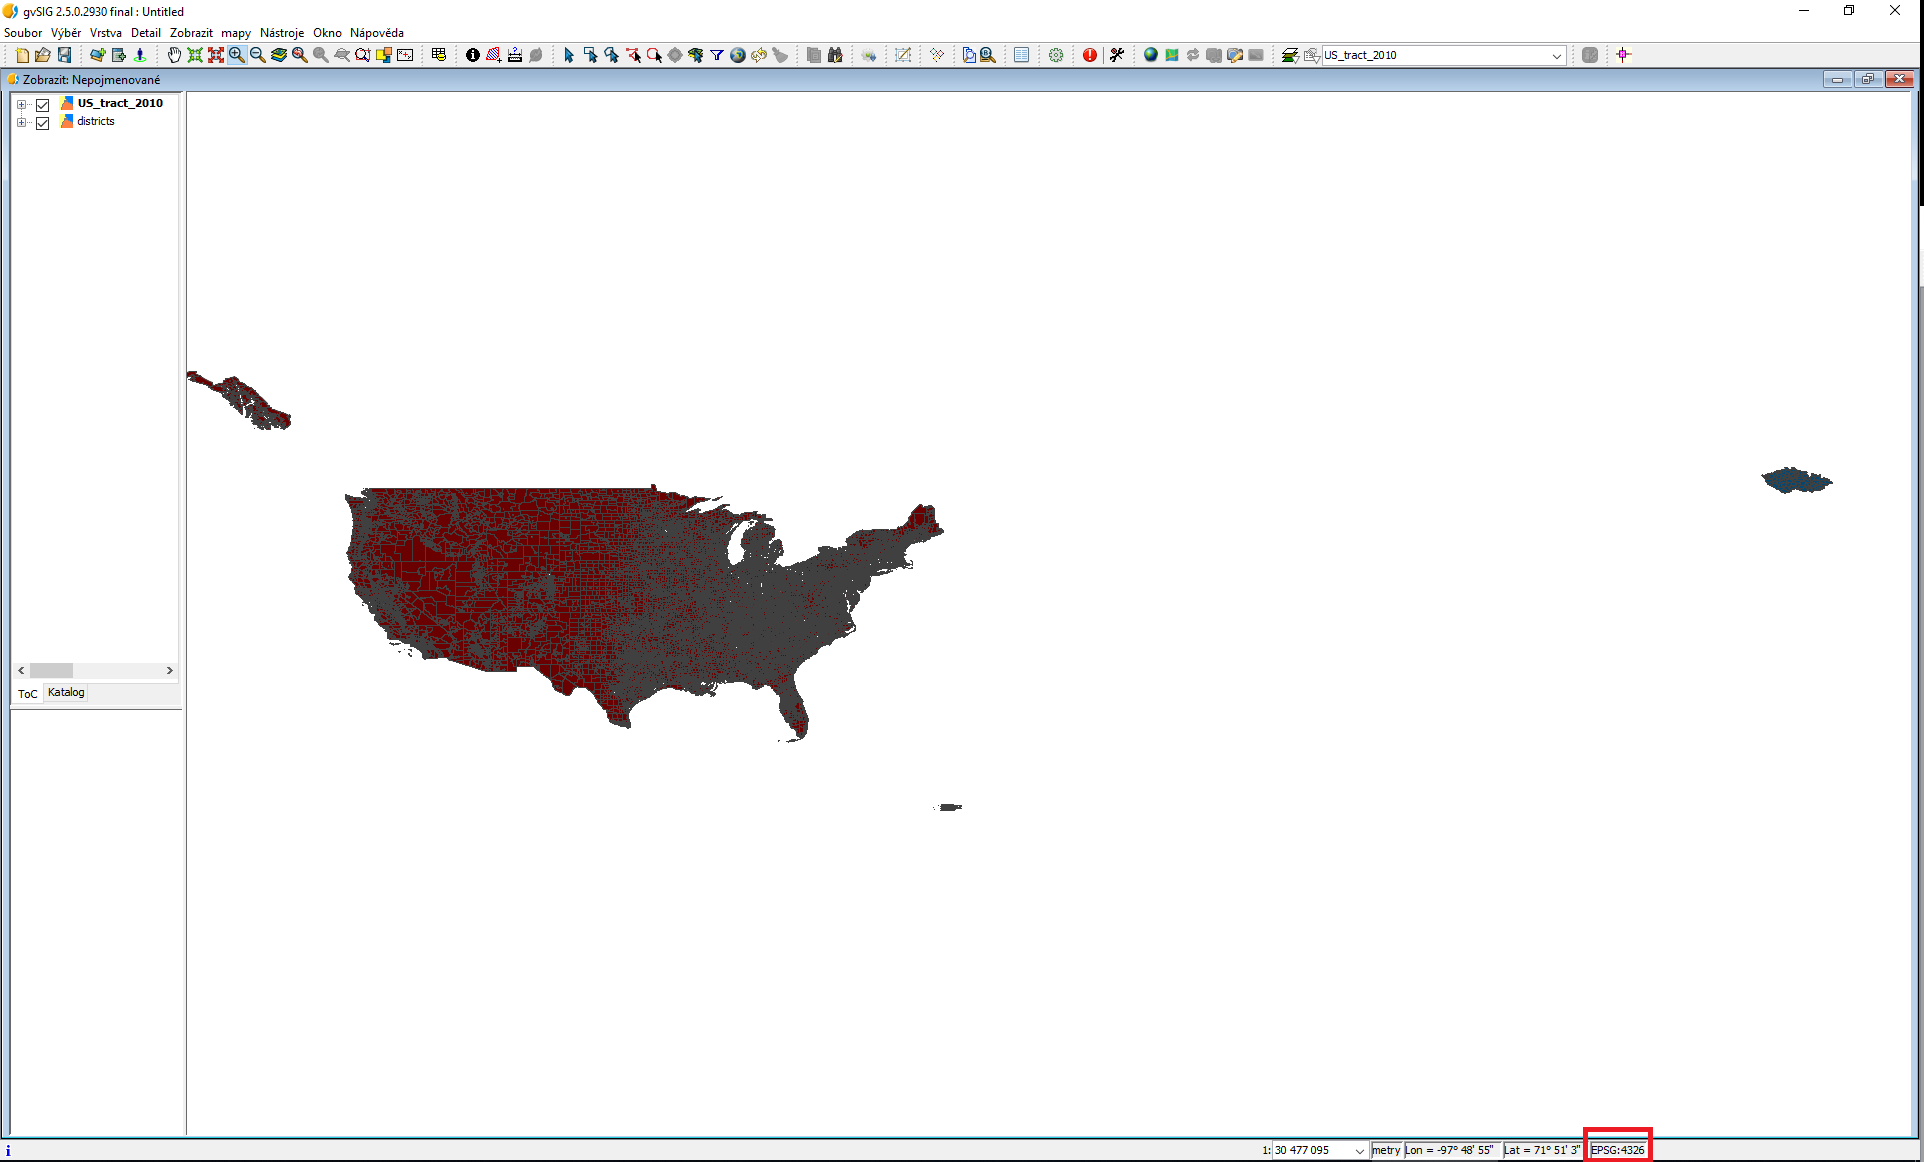
\includegraphics[width=17cm]{../pictures/gvSIG_coords.PNG} 
\caption[Correct display of layers with different coordinate system in gvSIG 2.5.0]{Correct display of layers with different coordinate system in gvSIG 2.5.0 (Source: Personal collection)}
\label{fig:gvSIG_coords}
\end{center}
\end{figure}

\newpage
\vspace*{-1cm} 
\bigskip
\noindent \textbf {ILWIS 3.3 (Integrated Land and Water Information System)}

\noindent The strong point of this system developed at University of Twente in the Netherlands has always been remote sensing and hydrological flow operations.

The software starts without a startup window and does not have features enhancing first-time user experience. On the left there is a section with several tabs: Operation-Tree, Navigator and Finder. ILWIS seems to be very similar to GRASS GIS. Operation-Tree and Finder are defacto the Modules tab in GRASS divided into two sub-tabs.  The data is similarly to GRASS stored in the home directory here called Data, which is taken as the default when importing or creating data. The content of this folder is in special formats that ILWIS understands, see Figure \ref{fig:ilwis_uvodni_okno}. 

The navigator has a tree structure like the GRASS Data Catalog and represents the entire directory structure, not just a home Data directory. ILWIS does not have its own native file to save the projects or workspaces.

\vspace{0.3cm}
\begin{figure}[hbt!] 
\begin{center}
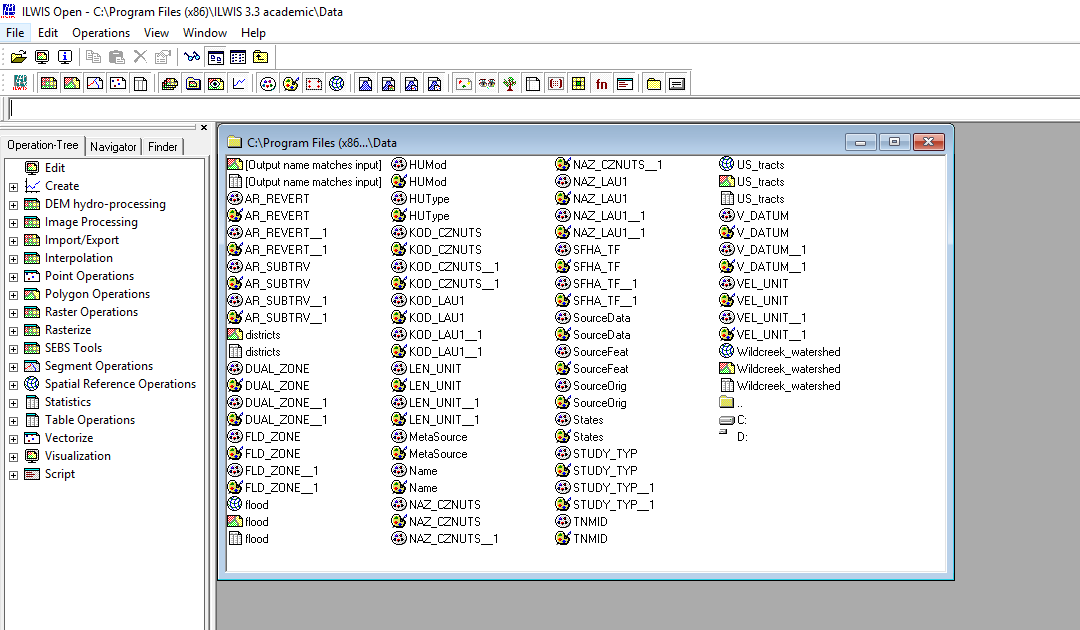
\includegraphics[width=17cm]{../pictures/ilwis_uvodni_okno.png} 
\caption[The main software window after reopening ILWIS 3.3]{The main software window after reopening ILWIS 3.3 (Source: Personal collection)}
\label{fig:ilwis_uvodni_okno}
\end{center}
\end{figure}

\noindent The display of layers with different coordinate system is tested as well. Importing data in the form of a shapefile is somewhat unintuitive here. If we want to perform an import we might go to the Operation-Tree $->$ Import/Export $->$ Import Map, however we encounter the problem that the software does not know the shapefile format. Therefore, the second option can be found in the top bar File $->$ Import. Here we select the ESRI shapefile and it is necessary to expand the default output so that the imported file is saved as an ILWIS object with the * .ioc extension. If we do not do this, only the tables will be imported, no maps.

It is interesting how the software approaches coordinate systems. When importing the layer called districts, the S-JTSK Krovak East North system is converted to the Unknown. In case of US tracts, the US Contiguous Albers Equal Area Conic system is converted to the LatLon system. Therefore, the software does not carry information about a specific coordinate system, it only cares about boundaries of the map. When displaying multiple layers with different coordinate systems in one map window, no On the fly transformation is performed. The system gets confused and the added layer is not displayed even after clicking on the ''Zoom to Layer'' function. There is no need to save the software, after opening it reflects the current state of the Data folder.

\vspace{0.3cm}
\begin{figure}[hbt!] 
\begin{center}
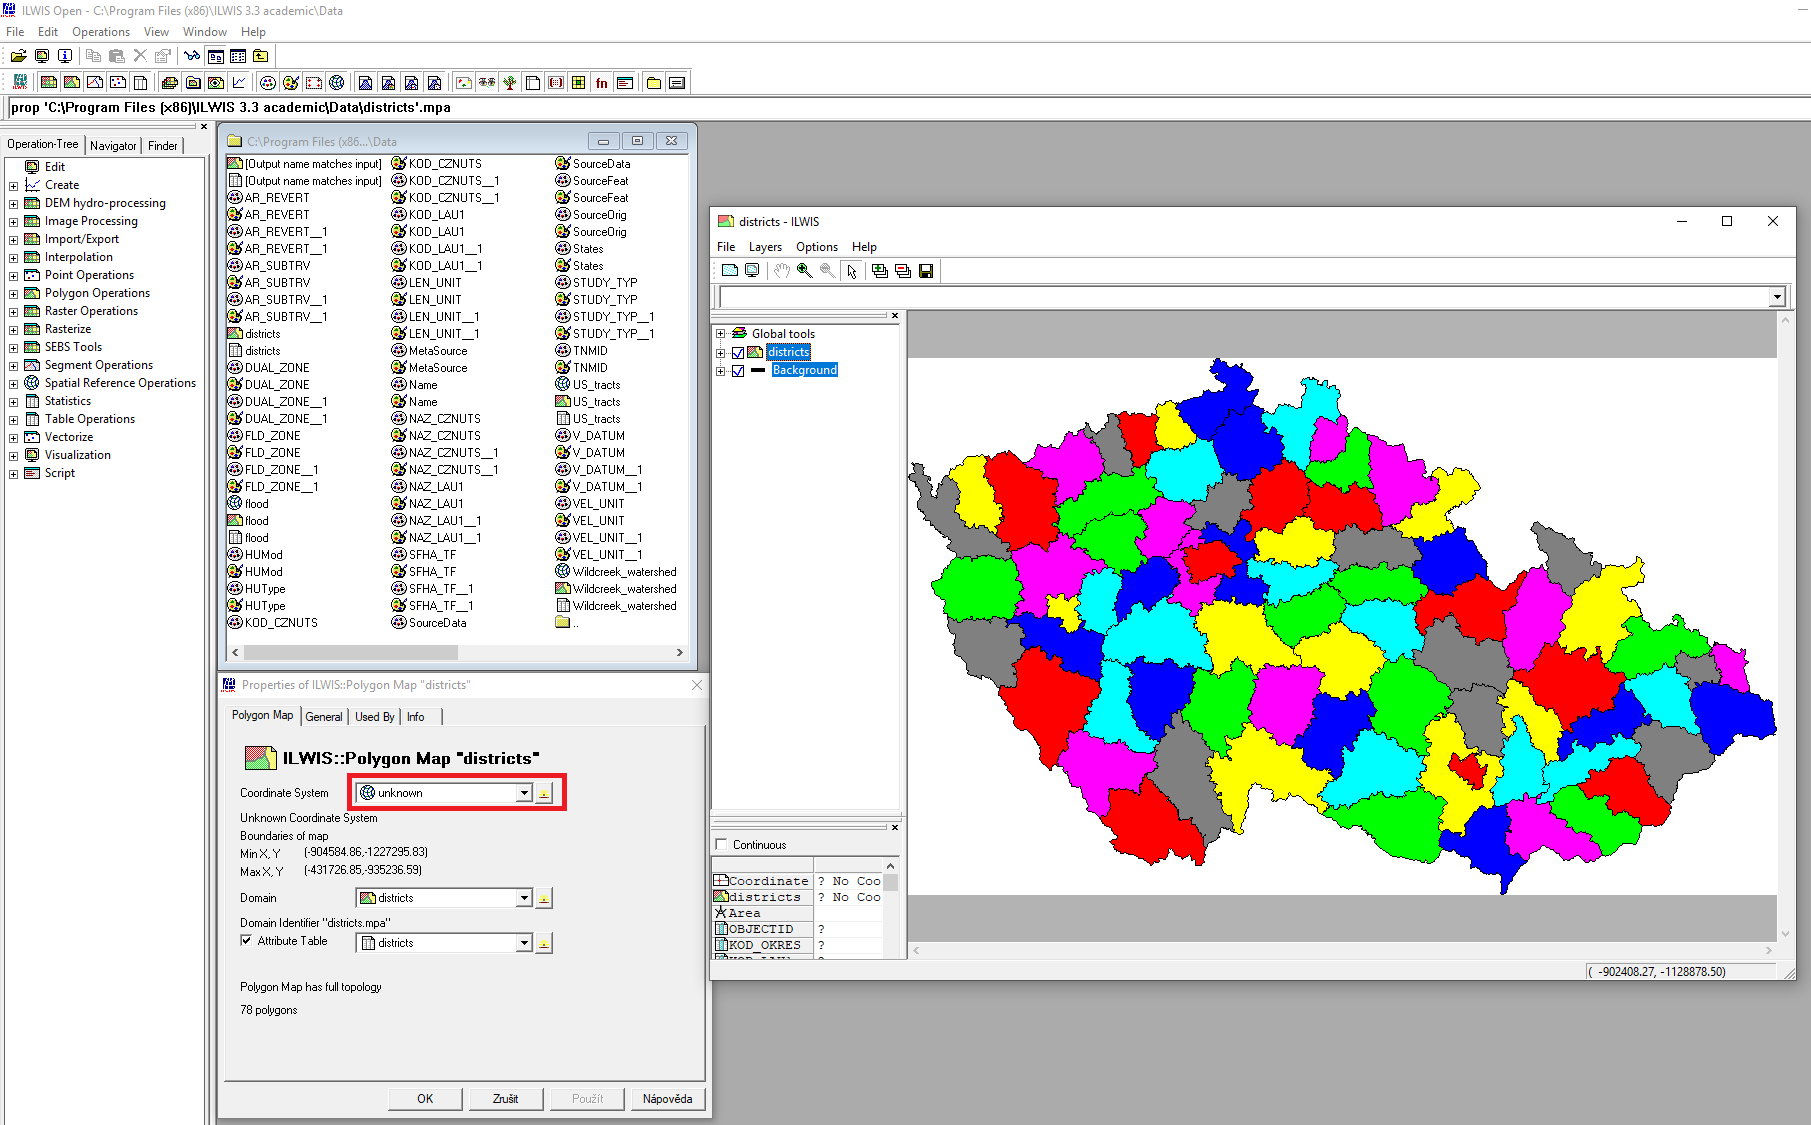
\includegraphics[width=17cm]{../pictures/ilwis_pridani_mapy.png} 
\caption[Unknown coordinate system properties of district layer in ILWIS 3.3]{Unknown coordinate system properties of district layer in ILWIS 3.3 (Source: Personal collection)}
\label{fig:ilwis_pridani_mapy}
\end{center}
\end{figure}

\bigskip

\noindent \textbf {SAGA GIS 2.3 (System for Automated Geoscientific Analyses)}

\noindent SAGA GIS is a Free Open Source Software (FOSS) offering a comprehensive, growing set of higher-level geoscientific methods. It is one of the most favorite software for remote sensing needs because of its rich library grid, imagery and terrain processing modules.

This software is blank the first time it is run. On the left there is a window with the Tools, Data and Maps tabs, which are similar to the Modules, Data, Layers tabs in GRASS GIS 7.8. The Data and Maps tabs are further divided into the Tree and Thumbnails subtabs. The tree is divided according to the shapes of geometric objects (point, line, polygon ...). 

The idea is different from GRASS GIS. The directory structure of added layers is always displayed for the current layer in the lower left window of Data Sources in the File System tab. So we do not have a specific folder in which we work from the beginning. We can add layers to the tree structure and the whole project will be created only when we save the settings to a SAGA GIS project file.

In the Maps tab, multiple layers can be displayed on top of each other or a new map map window can be created for each layer, which is a default option. However, there is no On the fly transformation. It means that layers with different coordinate systems may be displayed at the level of one map.  As we can see in Figure \ref{fig:saga_gis_cele}, the Czech Republic appears next to the American continent, as the system assumes adding layers with the same coordinate system to the map.

After the second start of SAGA GIS, a small selection dialog box will appear. We can run a blank page, the latest software state, or the last running projects sorted from newest to oldest (Figure \ref{fig:saga_startup}).

\vspace{0.3cm}
\begin{figure}[hbt!] 
\begin{center}
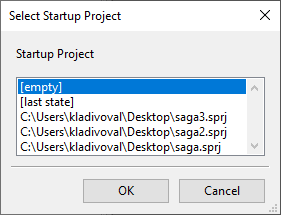
\includegraphics[width=6cm]{../pictures/saga_startup.png} 
\caption[Saga GIS 2.3 startup dialog]{Saga GIS 2.3 startup dialog (Source: Personal collection)}
\label{fig:saga_startup}
\end{center}
\end{figure}

\vspace*{-1cm} 
\subsubsection{Summary}
\label{subsec:startup_concepts_summary}

The summary corresponding to the questions asked at the beginning of this chapter is contained in the Figures \ref{fig:commercial_software} and \ref{fig:open-source_software}. In the cross-section of all selected GIS software, we can notice that the data hierarchy is quite different. The truth is that two world-famous representatives of GIS software - ArcGIS Pro and QGIS 3 -  have similar data organization into projects. However, in the data hierarchy of the other two commercial software GeoMedia and MapInfo, the term `` project '' does not appear at all. 

\newpage
\begin{figure}[hbt!] 
\begin{center}
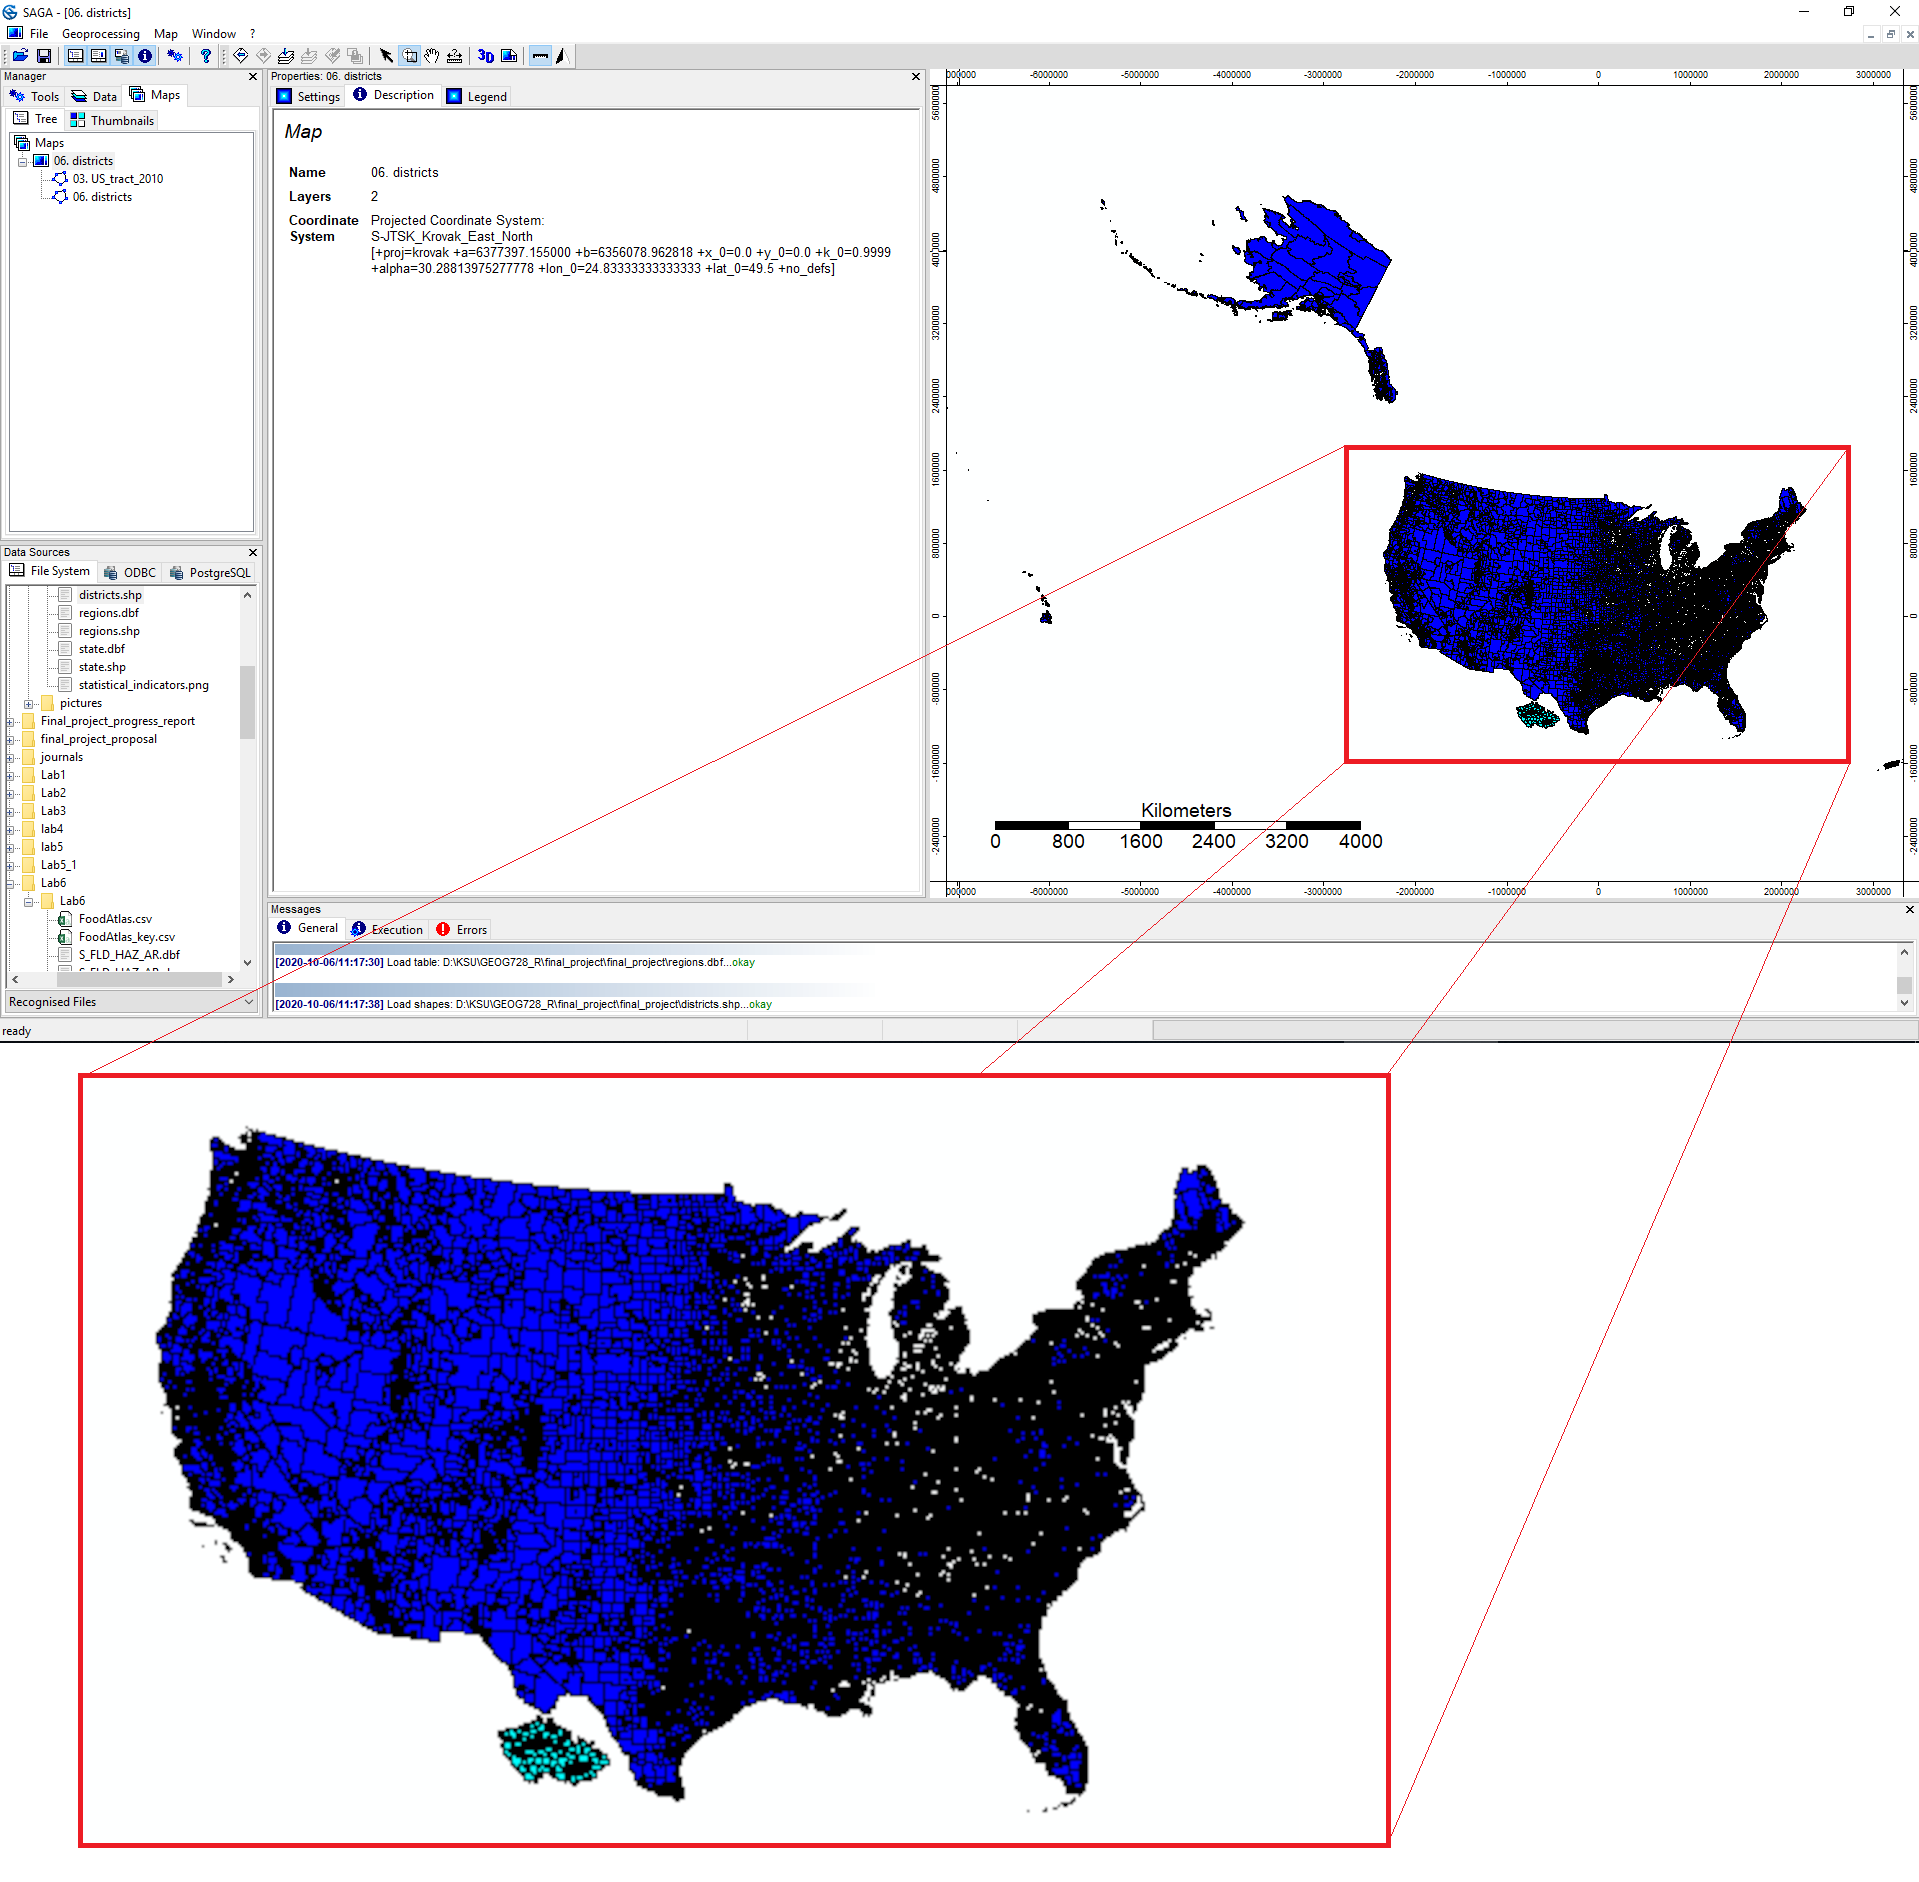
\includegraphics[width=17cm]{../pictures/saga_gis_cele.png} 
\caption[Incorrect display of layers with different coordinate system in SAGA GIS 2.3]{Incorrect display of layers with different coordinate system in SAGA GIS 2.3 (Source: Personal collection)}
\label{fig:saga_gis_cele}
\end{center}
\end{figure}

\noindent It is therefore good to realize that we may consider this name as a standard for data organization, especially for open-source software, but after looking at commercial software we find out that data organization across software is surprisingly different not only from a technical point of view, but also in terms of different names.

Startup screens appear in some form in all selected commercial software. For GeoMedia, it is a small dialog box whose purpose is purely organizational - choose the GeoWorkspace you will work in. For ArcGIS Pro and MapInfo, startup screens play a more important role. It tries to impress users with both modern design and the services they offer. Similarly, QGIS tries to make contact with the user from the beginning - it refers to news and displays Info Bars (see Fig. \ref{fig:qgis_warning_window}).

It is surprising how much of a difference there can be between commercial GIS software in terms of efforts to enhance the first-time user experience. With the GeoMedia software, the author did not manage to record any effort at all, on the contrary, MapInfo is very generous to its user from the very beginning and uses modern technologies in startup screen, such as videos on YouTube. Despite the fact that in some of selected software there is a certain effort to better interact with the initial user, none of them contains any first run wizard incorporated directly in the main software window (as offered by Zoner Photo Studio X, see the next chapter \ref{sec:other_software}). But this is not necessarily wrong. Whether any help at all makes sense and will not be rather counterproductive strongly depends on the complexity of data organization in a particular software. For example, with gvSIG software, there is no startup screen or any other helpful explanation, although it can be assumed that the new user will find his way around without any problems. GeoMedia also lacks any interactive features, however, as data organization is more complex to understand, it is likely to be much more inconvenient start for users.

As known, GRASS GIS went a different way from the beginning. Not only in data organization. The difference between GRASS and other GIS software goes far beyond the startup mechanism or data organization. Let's remember the unique Unix philosophy, where the software consists of a collection of small applications called modules, or the ability to call these modules from the command line. It is therefore interesting to note that the comparison of GRASS GIS with other GIS software does not provide significant inspiration for other implementations associated with the improvement of the startup mechanism, which requires (and probably deserves) a completely unique solution whose roots were laid already in the summer of 2020 by GSoC implementations. However, the comparison offers an interesting look at this topic, which is not talked about much, but certainly has a big impact on the whole software. The evidence may be, after all,  user complaints about the problematic startup screen in versions before GSoC.

We do not have to look for inspiration only in GIS software. How the software interacts with the first-time user is a completely general thing that plays a role in all types of software. In the next chapter, the author highlights several interesting cases of startup mechanisms involving user interaction. These are software that the author either uses herself or received a tip in the Quesion 4 from the second part of the survey number 1.

\vspace{0.3cm}
\begin{figure}[hbt!] 
\begin{center}
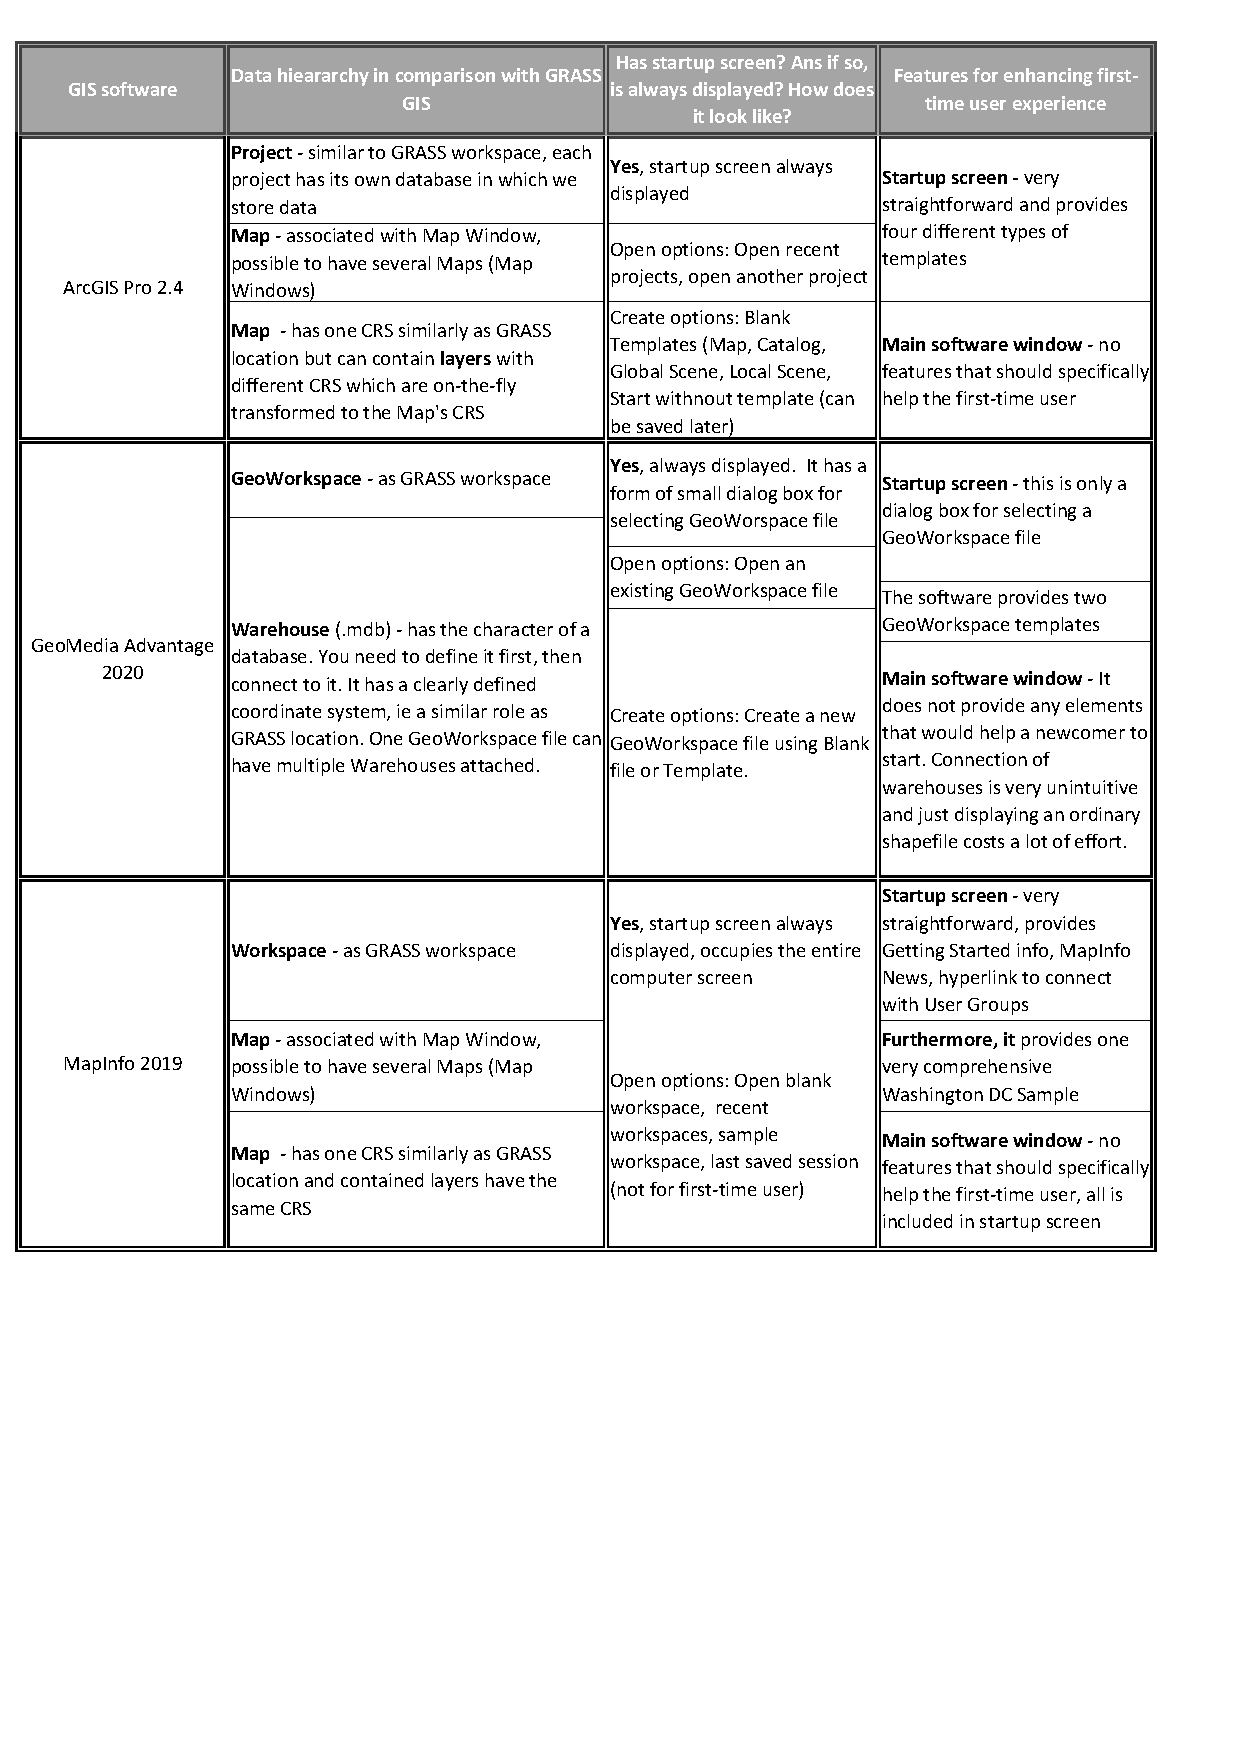
\includegraphics[width=15cm]{../pictures/commercial_software.pdf}
\caption[Analysis of selected commercial software]{Analysis of selected commercial software (Source: Personal collection)}
\label{fig:commercial_software}
\end{center}
\end{figure}

\vspace{0.3cm}
\begin{figure}[hbt!] 
\begin{center}
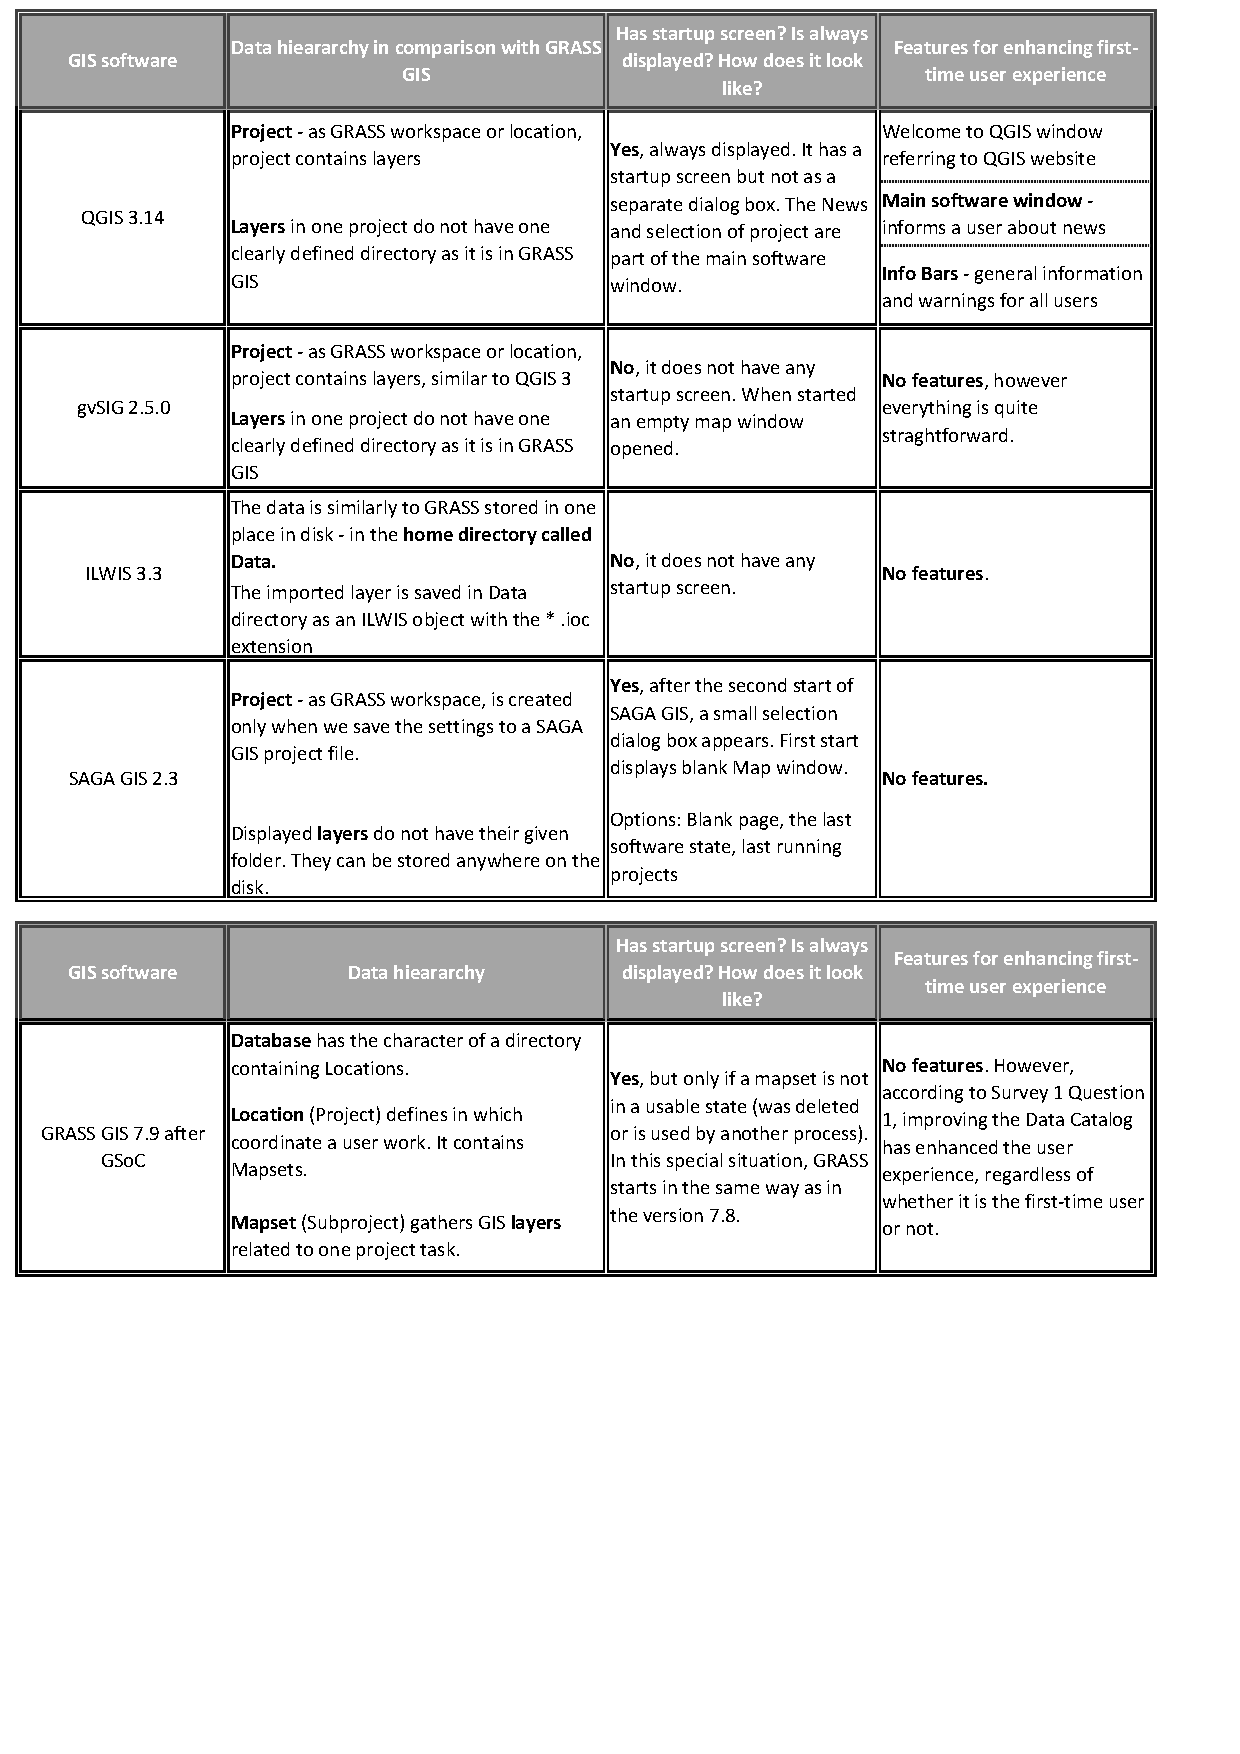
\includegraphics[width=15cm]{../pictures/open-source_software.pdf} 
\caption[Analysis of selected open-source software and GRASS GIS]{Analysis of selected open-source software and GRASS GIS (Source: Personal collection)}
\label{fig:open-source_software}
\end{center}
\end{figure}


\newpage
\vspace*{-1cm} 
\subsection{Interesting solutions from other software}
\label{sec:other_software}

\noindent \textit{\color{red}Dokončit!}

\noindent \textbf{Zoner Photo Studio X} \\

\noindent After the initial login and launching the main software window, a short first run wizard will appear and can be skipped. The guide consists of four parts. The first section introduces the main tabs on the left side of the software window called the Navigator and also explains the Catalog tab, which provides quick access to photos. The following are two pages of a guide describing photo thumbnails and zooming. The last page of the wizard lists the right toolbar and the three individual modules - Manager, Develop and Editor. The main software components described in the wizard are always marked with a blue frame and the individual information windows are assigned to a particular part by arrows. The wizard is not only at the beginning, but also when using the above-mentioned modules for the first time.

Images are managed in the Catalog, which has a tree structure. We edit the image, save it, and if we turn off the Zoner software and run it a second time, it starts up in the last opened file. If the last used file is deleted, the software is launched in the Manager tab in the last opened folder, where another image can be selected for editing or we can simply click to another folder and open or create another image. There is a native image format of Zoner Photo Studio X with extension * .zps, however, firstly, traditional formats such as * .jpg, * .png, * .tif, * .gif etc. are offered to us.

\vspace{0.3cm}
\begin{figure}[hbt!] 
\begin{center}
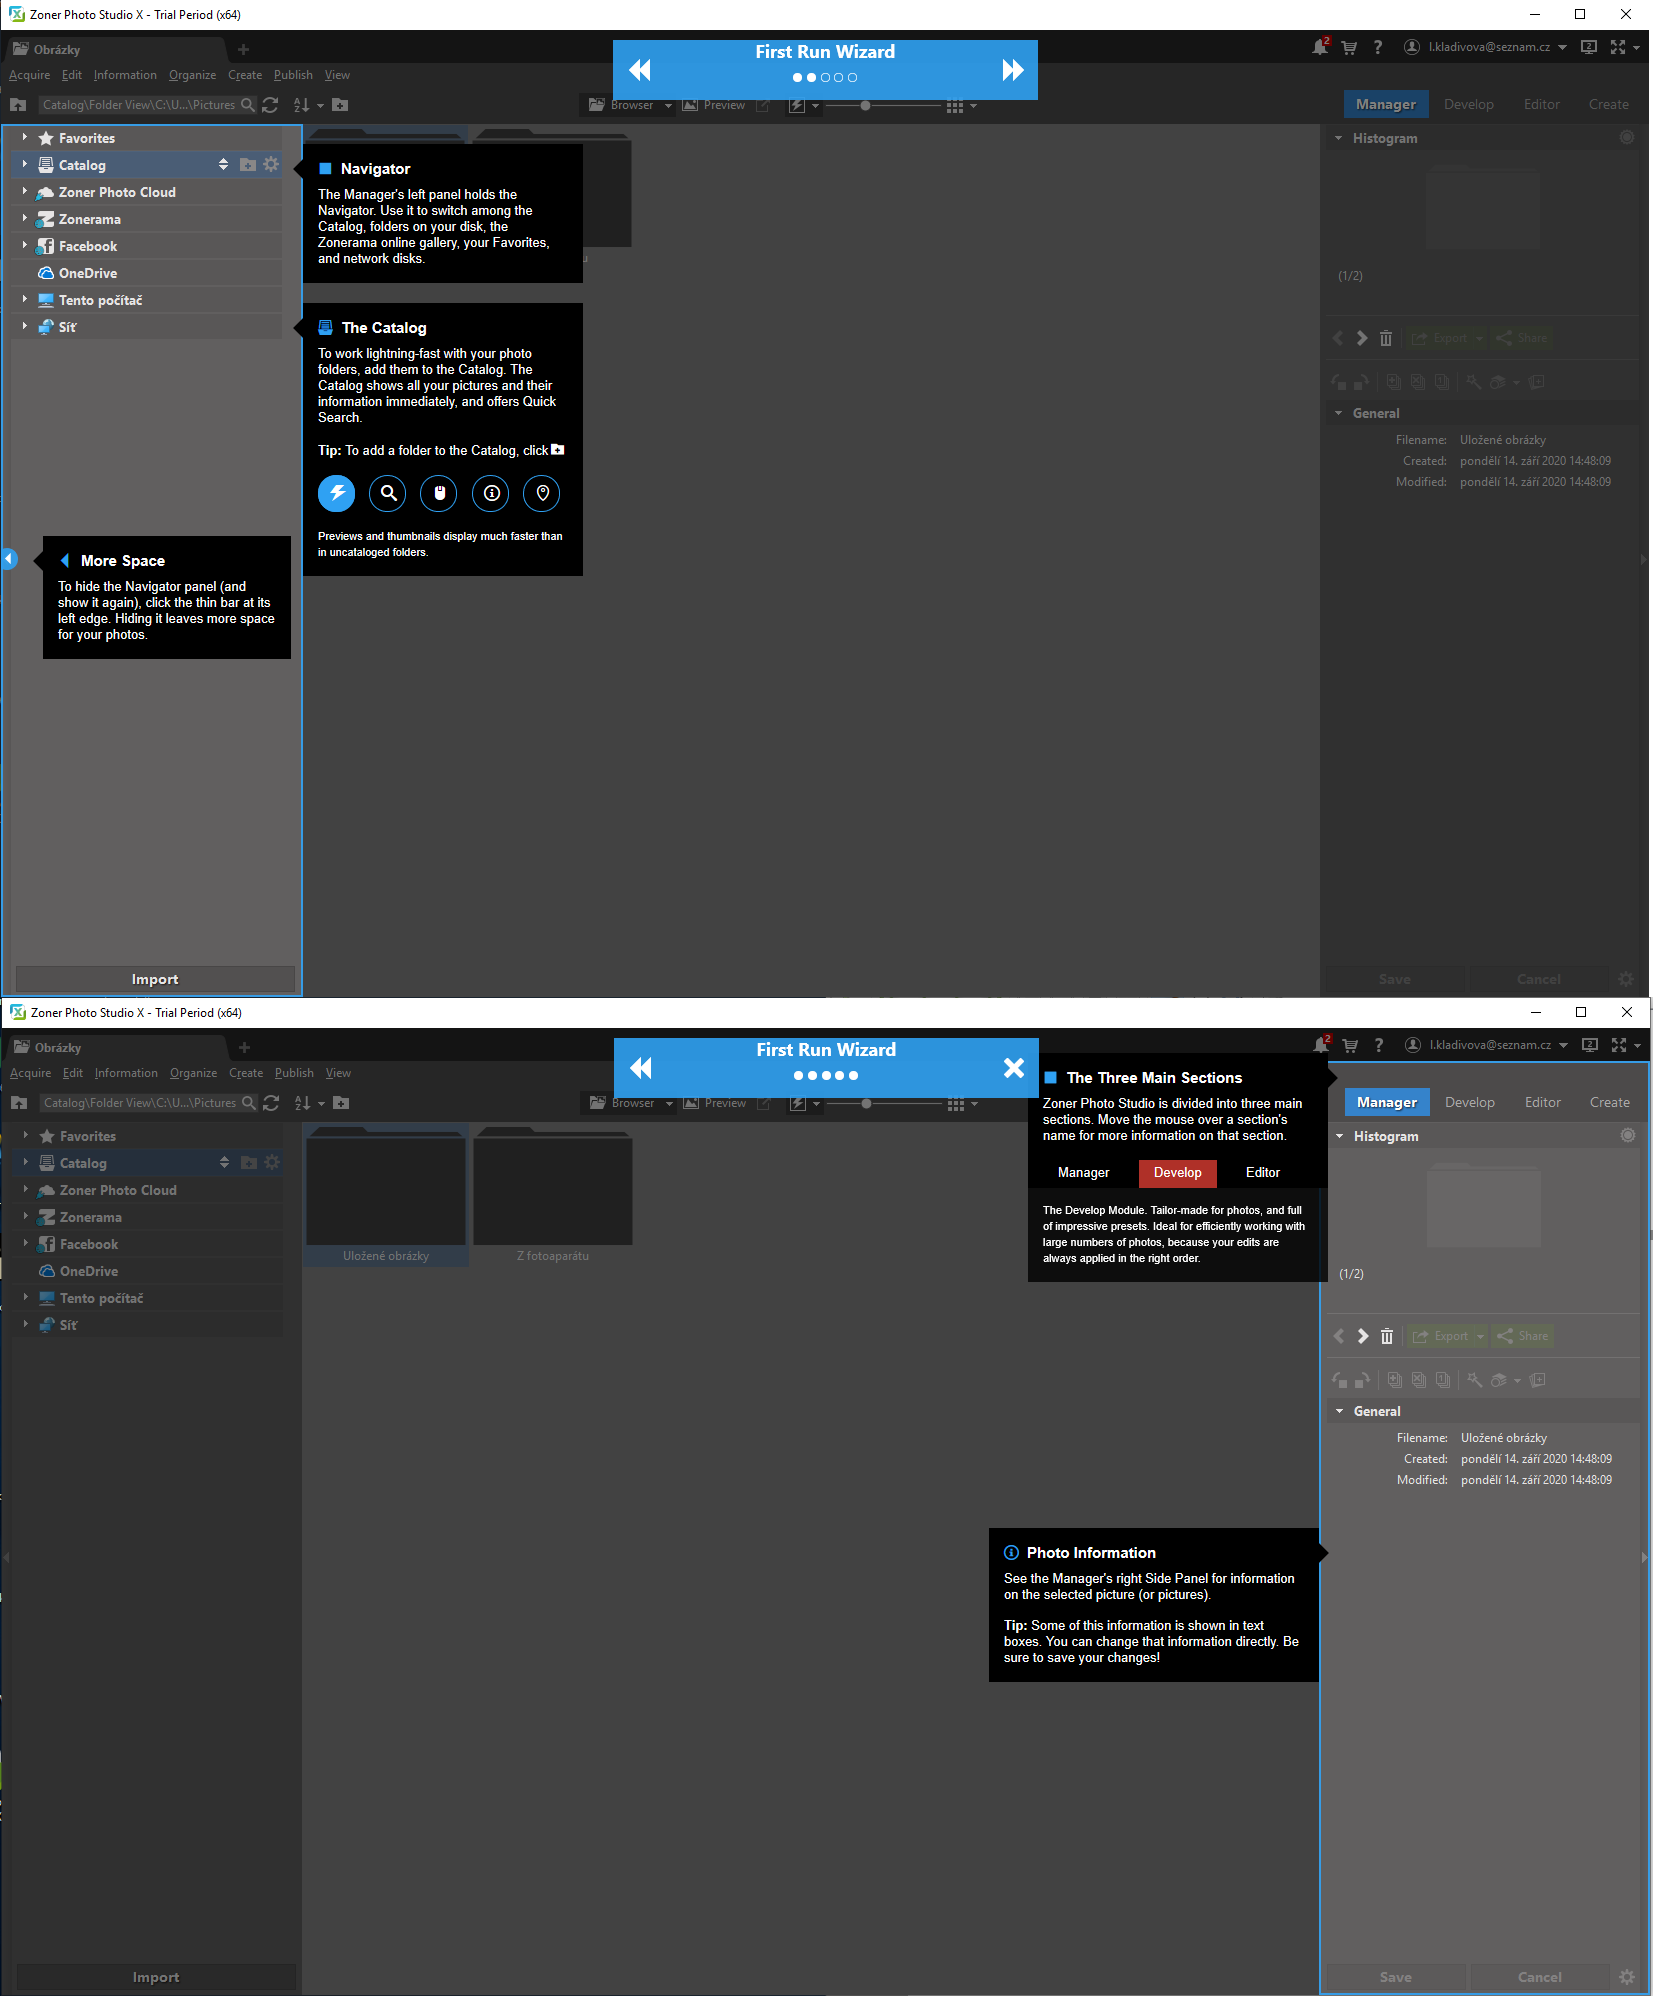
\includegraphics[width=15cm]{../pictures/zoner.png} 
\caption[First run wizard in Zoner Photo Studio X]{First run wizard in Zoner Photo Studio X}
\label{fig:zoner}
\end{center}
\end{figure}

\newpage
\vspace*{-1cm}
\subsection{Summary}

